\documentclass[10pt]{article}
\usepackage[letterpaper,margin=1in]{geometry}
\usepackage{booktabs}
\usepackage{amsmath}
\usepackage{graphicx}
\usepackage{placeins}
\usepackage{float}
\usepackage{url}
\usepackage{enumitem}
\setlength{\emergencystretch}{3em}
\title{Supplementary Material\\[2pt]
\large Temporal Referent Integrity: A Controlled Diagnostic of Referential Resolution Timing in Tool-Using Agents}
\author{Anonymous Submission}
\date{}

\begin{document}
\maketitle

\paragraph{Review note.}
This document supports the main submission with implementation, protocol, and extended-result
details. The main paper contains the complete argument; this document supplies extended results.
No result reported here changes the primary estimand. Literal prompts, complete runner interfaces,
inventories, raw outputs, and executable reports are in the separately uploaded anonymous Code and
Data Supplement rather than on an external webpage.

\newcommand{\PrimaryDiagnostic}{Matched Timing Diagnostic}
\newcommand{\NewSchemaReplication}{Cross-Schema Replication}
\newcommand{\GuardedExtension}{Action-Validity Stress Test}
\newcommand{\RuleStar}{Deterministic Rule*}

\section{Benchmark and Frozen Protocol}
The \PrimaryDiagnostic{} evaluation (internal inventory ID: TRI-v3) contains 160 tasks in 20 frozen language-template clusters.
Tasks are balanced across anchored and dynamic references and across flip, stable, remove,
invalidate, and name-collision transitions. The transfer evaluation contains 80 tasks over
four unseen schemas (projects, expenses, inventory, and cloud deployments). The
\GuardedExtension{} (internal inventory ID: TRI-v4) contains 40 conditional tasks and distinguishes action-validity and
selector-match guards. The model-facing SQLite trajectory experiment uses a frozen 40-task subset and
records every query, refresh, target proposal, mutation attempt, and final database diff.

The task generator evaluates the selector in $S_0$, applies a controlled transition to obtain
$S_1$, and computes the target from the instruction-conditioned resolution status. Each
task-specified resolver maps a state to one entity or $\bot$; the frozen generators construct a
unique eligible winner, and unresolved ranking ties are outside the inventory. At the refresh
boundary, Preserve induces a bound commitment $B(q(S_0))$, whereas Reevaluate retains an unresolved
query $U(q)$ for evaluation in $S_1$. This semantic status need not be serialized as an explicit
field. Paired items share their schema, entities, transition, and action; only temporal discourse
varies. Every controller receives the instruction's natural-language selector. Gold targets,
generator-normalized selector fields, and pre-/post-refresh winner IDs are not passed to the model.

\subsection{Evidence chronology and status}
The manuscript distinguishes the original primary comparison from later replication and audit
analyses. The chronology below prevents post-primary reanalyses from being read as preregistered
primary estimands.

\begin{table}[H]
\centering
\small
\begin{tabular}{p{0.22\textwidth}p{0.24\textwidth}p{0.42\textwidth}}
\toprule
Stage & Frozen status & Role in the manuscript \\
\midrule
\PrimaryDiagnostic{} & Primary/frozen before calls & Package-level Qwen Generic vs. Lifecycle-Gated estimand; GLM replication \\
\PrimaryDiagnostic{} component addenda & Post-primary; frozen before their own calls & Free actor, validity gate, mode-only, untyped-plan, and exact-CTA audits \\
\NewSchemaReplication{} & Post-primary replication; frozen before calls & New schemas and states; tests directional substitution \\
Matched full-history baselines & Post-primary strong baseline; frozen before own calls & Ordinary and final-step-aware history across three model families \\
Human construct labels & Post-primary construct validation & Three independent labels for each of 100 original/rewrite items \\
Human-rewrite model runs & Post-primary replication; frozen before own calls & Unchanged controllers on 50 volunteer rewrites \\
Full-diagnostic matched-call confirmation & Post-primary; frozen before own calls; complete & Equal calls and base actor payloads on all 160 diagnostic rows \\
Human-rewrite matched-call confirmation & Post-primary; frozen before own calls; complete & Equal-call transfer on 50 existing volunteer rewrites; model-dependent result \\
Source-derived matched-call contrast & Post-primary; frozen before own calls; complete & 30 changed pairs across three source-derived substrates and model families \\
40-task model-facing SQLite & Secondary/frozen execution test; GLM later replication & Model-issued mutations and final database states \\
\NewSchemaReplication{} deterministic replay & Post-primary, zero API & Consequence verification over frozen target outputs, not a new behavioral replication \\
PairAcc and identifiability & Post-primary, zero API & Matched, marginal, and shared-eligible reanalyses of frozen outputs \\
Crossed-dependence sensitivity & Post-primary, zero API & Domain, template, and two-way resampling of the primary package contrast \\
Call/information-matched ablation & Post-primary; both models complete & Shared compiler call and matched actor payloads; explicit-decision and enforcement contrasts \\
Selection regret & Post-primary, zero API & Proxy maximizers and changed-PairAcc regret in frozen candidate sets \\
Model-authored linguistic audit & Post-primary; transport-repaired & 24 generated pairs; two model judges jointly validate no complete pair \\
Strengthened deterministic rule & Post-hoc & Benchmark-aware deterministic audit after first-rule failure inspection \\
Public-suite audits & Post-primary/descriptive & Coverage checklist for audited ToolSandbox, AppWorld, and $\tau^3$-Bench versions \\
Injected audit sensitivity & Post-primary, zero API & Known-positive and one-feature-missing controls; implementation check only \\
Model-assisted recall triage & Post-primary, zero API & Candidate-label queue over six public suites; not independent recall calibration \\
Source-anchored external transfer & Post-primary; frozen before calls & Author-adapted matched contrast on pinned STATE-Bench and AgentDojo states and source tools \\
\bottomrule
\end{tabular}
\caption{Evidence status used throughout the paper. Planned or unverified analyses are not
reported as results.}
\label{tab:supp-chronology}
\end{table}

\begin{figure}[H]
\centering
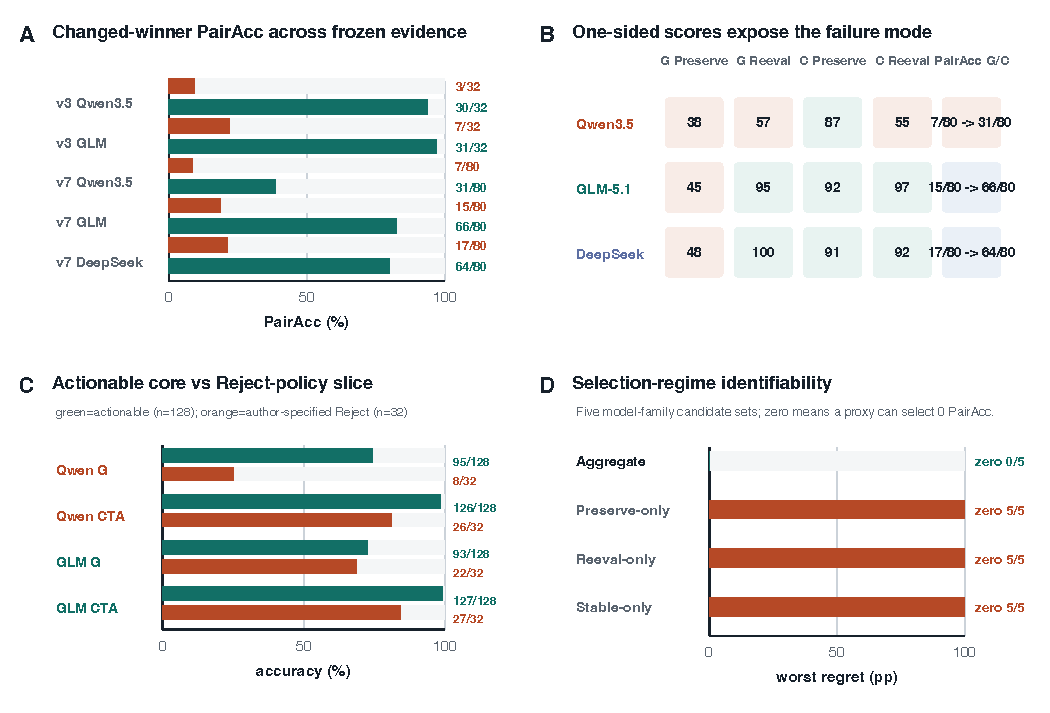
\includegraphics[width=0.98\textwidth]{Figures/tri_comprehensive_results.pdf}
\caption{Post-primary audits from frozen \PrimaryDiagnostic{} and \NewSchemaReplication{} outputs.
\textbf{(A)} Changed-winner PairAcc for Generic and historical CTA on 32 v3 and 80 v7 pairs.
\textbf{(B)} V7 one-sided mode accuracies and complete-pair accuracy (G/C: Generic/CTA).
\textbf{(C)} V3 actionable-core accuracy versus the author-specified Reject-policy slice; human
support is weaker for Reject. \textbf{(D)} Worst changed-PairAcc selection regret across five
model-family candidate sets; ``zero'' counts regimes whose maximizers include a zero-PairAcc policy.}
\label{fig:supp-comprehensive-results}
\end{figure}

\subsection{Diagnostic matrix and metric roles}
The actionable referential core crosses authorization with whether the selector winner changes.
This separates structural sensitivity from success caused by an unconditional policy.
Remove and Invalidate are retained as a separate execution-policy slice because Preserve may
correctly yield \textsc{Reject} rather than an entity ID.

\begin{table}[H]
\centering
\small
\begin{tabular}{llll}
\toprule
Authorization & Transition & Gold target & Diagnostic role \\
\midrule
Preserve & Stable & $q(S_0)=q(S_1)$ & Ordinary-execution control \\
Reevaluate & Stable & $q(S_1)=q(S_0)$ & Detect refresh overreaction \\
Preserve & Changed winner & $q(S_0)$ & Detect temporal rebinding \\
Reevaluate & Changed winner & $q(S_1)$ & Detect unconditional locking \\
Preserve & Remove/Invalidate & $\bot$ by policy & Validity/fallback compliance \\
Reevaluate & Remove/Invalidate & $q(S_1)$ & Valid reselection control \\
\bottomrule
\end{tabular}
\caption{Complementary condition design. ``Changed winner'' comprises Flip and name collision;
paired rows keep both states, selector, action, schema, and update fixed.}
\label{tab:supp-diagnostic-matrix}
\end{table}

\subsection{Restricted policy-identifiability result}
Let $L$, $R$, and $S$ denote Always-Lock, Always-Reevaluate, and Selective policies. Consider
changed-winner contexts with shared $(S_0,S_1,q,a)$, old winner $e=q(S_0)$, refreshed winner
$e'=q(S_1)$, and $e\neq e'$. A Preserve row has gold $e$ and a Reevaluate row has gold $e'$.

\paragraph{Observation.}
For the policy class $\{L,R,S\}$, an exact-target evaluation identifies $S$ against both $L$ and
$R$ only if it contains at least one changed Preserve row and at least one changed Reevaluate row.
A matched opposite-gold pair is sufficient and has minimum cardinality two.

\paragraph{Argument.}
If the evaluation contains no changed Preserve row, $R$ and $S$ agree on every Reevaluate row and
on every Stable row, so they are observationally equivalent. If it contains no changed Reevaluate
row, the same argument makes $L$ and $S$ observationally equivalent. Thus both authorization
directions are necessary. On a matched changed pair, $L$ outputs $e$ twice and fails Reevaluate;
$R$ outputs $e'$ twice and fails Preserve; $S$ outputs $(e,e')$ and can pass both. One row cannot
contain both authorization directions, so two rows are minimal. The statement is restricted to
these policy alternatives and exact-target observations; it is not a lower bound for arbitrary
stochastic controllers.

Exact target accuracy measures end-to-end task success but can hide complementary errors.
For $N$ complete pairs, we therefore report
\[
\mathrm{PairAcc}=\frac{1}{N}\sum_{i=1}^N
\mathbf{1}[\hat y_i^P=y_i^P\;\wedge\;\hat y_i^R=y_i^R].
\]
Preserve and Reevaluate marginal accuracy expose which side fails; PairAcc requires both members
to be correct. API, parse, protocol, and missing-output rows are incorrect under intention to
treat. Conditional substitution then isolates a narrower mechanism: among changed-winner Preserve
rows, the initial ID must be observably correct and remain present and action-valid before
substitution to the distinct refreshed winner enters the numerator. This numerator counts
violations, not successful preservation of TRI. Wrong writes, invalid attempts, and
unnecessary rejection are separate execution outcomes, not aliases for target accuracy.

\begin{figure}[h]
\centering

\includegraphics[width=0.72\textwidth]{Figures/tri_authorization_tradeoff.pdf}
\caption{Preserve versus Reevaluate accuracy on the 32 frozen \PrimaryDiagnostic{} changed-winner pairs. Each
model/controller point is labeled with PairAcc (P). The unconditional controls occupy opposite
corners, while high joint performance requires the upper-right region. Coincident Qwen/GLM
Lifecycle-Gated points are combined. \RuleStar{} is post-hoc. Values are generated from the same raw
runs as the matched-pair tables.}
\label{fig:supp-authorization-tradeoff}
\end{figure}

\begin{table}[H]
\centering
\small
\begin{tabular}{p{0.29\textwidth}p{0.34\textwidth}p{0.29\textwidth}}
\toprule
Question & Evidence & Supported conclusion \\
\midrule
Stable Preserve/Reevaluate semantics & Blind labels and independent rewrites & Core scalar construct supported; reject fallback weaker \\
Substitution after correct binding & \PrimaryDiagnostic{}/\NewSchemaReplication{} conditional audits, three models & Occurs for tested controllers under controlled conditions \\
Refreshed-winner direction & Flip, Stable, and name-collision controls & Supports a controller-level diagnosis, not random error \\
Executed consequence & Deterministic SQLite replay & Can cause wrong-entity mutation \\
Dependence on CTA & CTA, Lifecycle, and post-hoc \RuleStar{} & No uniquely necessary implementation \\
External-style occurrence & Mixed ToolSandbox-compatible audits & Limited and not reproduced at lower intervention \\
Public benchmark coverage & ToolSandbox, AppWorld, and $\tau^3$-Bench audits & Zero strict native opportunities in audited versions \\
Natural prevalence & No uncontrolled traffic evidence & Not estimated \\
\bottomrule
\end{tabular}
\caption{Evidence boundary. Each row separates the completed evidence from the strongest
conclusion it supports.}
\label{tab:supp-evidence-boundary}
\end{table}

\FloatBarrier

\section{Controller Records}
Executable resolution status and transition authorization are the design principle. Historical CTA is the minimal scalar
pre-refresh commitment implementation and has no deterministic gate. Lifecycle adds a typed,
auditable validity/fallback record; Lifecycle-Gated enforces that record at mutation time.
The Generic pipeline passes the original instruction separately to its actor; its compiled
ledger stores the initial selected ID, full entity snapshot, selector, requested action, and
action preconditions. It omits
reference mode and invalidity/fallback semantics. The scalar Lifecycle compiler additionally
emits \texttt{reference\_mode}, \texttt{bound\_target\_id}, \texttt{selector}, and
\texttt{invalidity\_policy}. A deterministic executor checks action validity for preserved
identities and delegates only explicitly dynamic or unresolved branches to the actor. The
separate \GuardedExtension{} adds \texttt{guard\_type} and
\texttt{fallback\_policy}; these fields are not part of the scalar \PrimaryDiagnostic{} record. The exact
historical Compile-then-act baseline is retained unchanged as a neighboring audit.

The \GuardedExtension{} guards are deterministic. Under \texttt{action\_validity}, the controller retains the
old ID iff all action preconditions $V_a(e_0,S_1)$ hold; otherwise it reevaluates $q(S_1)$.
Under \texttt{selector\_match}, it retains the old ID iff it is action-valid and remains
$q(S_1)$; otherwise it reevaluates. The frozen 40-task inventory crosses two guard types, five
instruction templates per guard, four unseen schemas, and scheduled transition types. Qwen Generic
scores 21/40 (52.5\%) and Lifecycle-Gated 34/40 (85.0\%); this secondary extension is not part of
the primary comparison. Complete task rows and the source-derived report are in the Code and Data Supplement.

\subsection{Lifecycle-Gated procedure}
\begin{table}[H]
\centering
\small
\setlength{\tabcolsep}{4pt}
\begin{tabular}{rp{0.82\textwidth}}
\toprule
& Lifecycle-Gated execution \\
\midrule
1 & Observe $S_0$ and compile $L(r,a)$ from the instruction and action schema. \\
2 & Execute the required environment refresh and receive $S_1$. \\
3 & If mode is \textsc{Preserve}, check the compiled bound ID against $V_a$. \\
4 & If valid, emit the bound ID without invoking the actor. \\
5 & If invalid, apply the compiled reject or reselection fallback. \\
6 & For \textsc{Reevaluate} or unresolved conditional branches, invoke the actor on $L(r)$ and $S_1$. \\
\bottomrule
\end{tabular}
\caption{Controller procedure. The instruction supplies the natural-language selector; gold,
generator-normalized selector fields, and winner IDs are never provided to the compiler or actor.}
\label{tab:supp-procedure}
\end{table}

\subsection{Information and execution audit}
\begin{table}[h]
\centering
\small
\begin{tabular}{llll}
\toprule
Controller & Pre-refresh output & Calls & Gate\\
\midrule
Generic ledger & ID, snapshot, selector, action, preconditions & 2 & no\\
Untyped plan & free-form plan & 2 & no\\
Historical CTA & binding time, ID, selector, reason & 2 & no\\
Lifecycle free & mode, ID, selector, policy & 2 & no\\
Lifecycle-Gated & same typed record & 1 or 2 & yes\\
\bottomrule
\end{tabular}
\caption{The gated Preserve branch omits the actor call. Generic retains all task-relevant
evidence and is not an information-deletion baseline.}
\end{table}

Untyped-plan and Lifecycle-free both compile before refresh, use two calls, share the action
schema and actor, and differ in whether the intermediate contract is free-form or typed.
Historical CTA is not a pure representation match: its actor omits the action schema and its
Preserve rule rejects only missing, rather than present-but-invalid, entities.

\subsection{Executor-level oracle check}
\begin{table}[h]
\centering
\small
\begin{tabular}{lrl}
\toprule
Generator-supplied representation & Accuracy & Characteristic failure\\
\midrule
Bound ID only & 41.9 & premature binding\\
Binding time only & 58.1 & no anchored identity\\
Bound name only & 58.9 & alias/name collision\\
Latest state & 64.6 & temporal rebinding\\
Time + ID & 74.0 & invalidity/conditional policy\\
Full lifecycle schema & 100.0 & --\\
\bottomrule
\end{tabular}
\caption{Deterministic execution over 246 generated tasks. This establishes sufficiency for
generated semantics only, not model performance, minimality, or natural-language validity.}
\end{table}

\section{Extended Component Audit}
The intervention ladder is interpreted through alternatives it can rule out, not by assuming that
every added component is necessary. The principal comparisons are:

\begin{figure}[h]
\centering
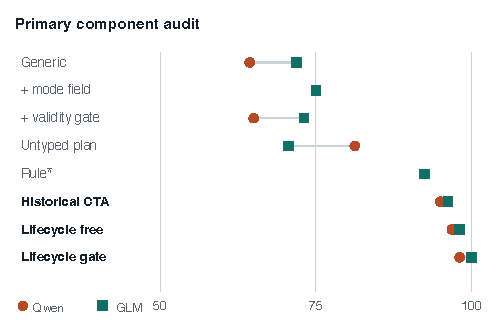
\includegraphics[width=0.78\textwidth]{Figures/tri_component_audit_dotline.pdf}
\caption{Component audit on \PrimaryDiagnostic{} exact-target accuracy. The dot-line format
shows the same controller sequence for Qwen and GLM without implying that any single component is
a causal estimate of the full package.}
\label{fig:supp-component-audit}
\end{figure}

\begin{table}[h]
\centering
\small
\begin{tabular}{p{0.25\textwidth}p{0.32\textwidth}p{0.34\textwidth}}
\toprule
Comparison & Alternative explanation tested & Result that would weaken the TRI interpretation \\
\midrule
Generic vs. full history & Missing task evidence & Full history removes changed-winner substitution \\
Always-Lock vs. Always-Reevaluate & One fixed update policy suffices & Either extreme succeeds on both pair members \\
Stable vs. changed winner & Generic refresh instability & Comparable errors without a winner change \\
Validity gate vs. Generic & Action validity alone identifies the referent & Gate removes valid-target substitutions \\
Untyped plan vs. typed lifecycle & Any extra pre-refresh computation suffices & Call-matched plan closes the lifecycle gap \\
CTA/lifecycle vs. \RuleStar{} & A learned or complex method is necessary & Deterministic discourse rule matches them \\
Target choice vs. SQLite replay & Errors are only representational & Substitutions do not change executed entities \\
\bottomrule
\end{tabular}
\caption{Falsification role of completed controls. A failed alternative does not prove a unique
internal mechanism; it narrows the controller-level behavioral explanation.}
\label{tab:supp-intervention-logic}
\end{table}

\begin{table}[h]
\centering
\small
\begin{tabular}{lrr}
\toprule
Controller & Qwen3.5 & GLM-5.1\\
\midrule
Generic free actor & 64.4 & 71.9\\
Generic + reference mode & 75.0 & 75.0\\
Generic + validity gate & 65.0 & 73.1\\
Untyped pre-refresh plan & 81.2 & 70.6\\
\RuleStar{} (post-hoc) & 92.5 & 92.5\\
Historical CTA & 95.0 & 96.2\\
Lifecycle free actor & 96.9 & 98.1\\
Lifecycle-Gated & 98.1 & 100.0\\
\bottomrule
\end{tabular}
\caption{Exact target accuracy on the identical 160-task language set.}
\end{table}

\subsection{Handcrafted discourse-rule audit}
The rule controller is intentionally non-neural. At prediction time it reads only the instruction,
$S_0$, $S_1$, and action schema. It locates selection and refresh events in the instruction,
uses event order to choose Preserve or Reevaluate, resolves the selector in the corresponding
state, and applies action preconditions to a preserved ID. It cannot read the benchmark
\texttt{binding}, \texttt{selector}, \texttt{update}, \texttt{style}, gold target, pre/post target,
new leader, CTA record, or any model output.

\begin{table}[h]
\centering
\small
\setlength{\tabcolsep}{4pt}
\begin{tabular}{lrrr}
\toprule
Rule & Timing diagnostic (160) & Human rewrites (50) & Schema replication (240)\\
\midrule
Naive rule, frozen & 60.6 & 74.0 & 77.5\\
\RuleStar{}, post-hoc & 92.5 & 96.0 & 91.7\\
\bottomrule
\end{tabular}
\caption{Exact authorized-target accuracy (\%). The naive rule was frozen before complete-set
execution. \RuleStar{} was written after inspecting its failures across these inventories and is a
strong benchmark-aware post-hoc baseline, not held-out generalization evidence.}
\label{tab:supp-rule}
\end{table}

The naive rule leaves 52/160, 12/50, and 44/240 items unresolved. \RuleStar{} adds the observed event
vocabulary and handles a single action-valid candidate without requiring a ranking field. No
further changes are made after this post-hoc revision. Its frozen source SHA-256 is
\texttt{34cbbd39072b...1bbfb8}; the complete digest is in the artifact manifest. On
\PrimaryDiagnostic{}, CTA minus \RuleStar{} is +2.5 points for Qwen and +3.8 for
GLM, with both cluster intervals spanning zero. On \NewSchemaReplication{}, \RuleStar{} exceeds Qwen CTA and is statistically
tied with GLM and DeepSeek CTA. Thus the benchmark does not require a uniquely learned algorithm.
The defensible commonality is an executable transition-authorization decision; the rule does not
show that a fixed lexicon generalizes to unrestricted instructions.

After recording source SHA-256 \texttt{34cbbd39072b...1bbfb8}, we applied the unchanged rule to
the 30-pair source-derived inventory frozen on STATE-Bench, AgentDojo, and ToolSandbox states and
schemas. It reaches 15/60 row accuracy and 2/30 PairAcc. Table~\ref{tab:supp-rule-source} keeps the
source failures visible; this application is held out from Rule* development but remains a
post-hoc rule evaluated on author-adapted controlled contrasts.

\begin{table}[H]
\centering
\small
\begin{tabular}{lrrl}
\toprule
Source & Rows correct & PairAcc & Dominant failure \\
\midrule
STATE-Bench & 9/20 & 0/10 & extra numeric field / wrong target \\
AgentDojo & 0/20 & 0/10 & unsupported timestamp selector \\
ToolSandbox & 6/20 & 2/10 & ranking cue absent / wrong target \\
\midrule
All & 15/60 & 2/30 & -- \\
\bottomrule
\end{tabular}
\caption{Frozen Rule* transfer to three source-derived controlled contrasts. The rule source and
task inventory are hash-locked before this zero-API application. These are not native benchmark
tasks or a learned-versus-rule causal comparison.}
\label{tab:supp-rule-source}
\end{table}

The benchmark-aware Rule* misses 20/240 \NewSchemaReplication{} rows, evenly split between
Preserve and Reevaluate. A post-hoc zero-API residual audit evaluates frozen full-history and CTA
outputs only on those rows.

\begin{table}[H]
\centering
\small
\begin{tabular}{lrrr}
\toprule
Model & History-only & Timing-reminder & CTA \\
\midrule
Qwen & 10/20 & 13/20 & 13/20 \\
GLM & 10/20 & 20/20 & 20/20 \\
DeepSeek & 15/20 & 18/20 & 16/20 \\
\bottomrule
\end{tabular}
\caption{Exact-target accuracy on rows missed by post-hoc Rule*. Selection uses observed Rule*
errors and leaves zero complete Preserve/Reevaluate pairs, so PairAcc is undefined and these row
accuracies are descriptive. The audit provides no residual CTA advantage over Timing-reminder.}
\label{tab:supp-rule-hard-residual}
\end{table}

\subsection{Concurrent Binding Drift baseline adaptation}
Binding Drift (Babu and Indukuri 2026, arXiv:2607.18316) studies a primary carry slot whose gold
entity remains constant across later workflow steps, together with entity-lock and LLM
re-verification defenses. We audited public commit
\texttt{0e040e0954b18d4621a6f9b16f6e6e9591c822e1}. Its deterministic offline harness passes
25/25 assertions after mapping the current 200-workflow file to the legacy filename expected by the
test script; the clean checkout otherwise raises \texttt{FileNotFoundError}. This path repair and
the adaptation below are recorded separately.

The post-primary author adaptation applies entity-lock semantics and the public LLM
self-reverification prompt frame to all 240 actionable \NewSchemaReplication{} rows. The verifier
receives the complete temporal instruction and refreshed candidates. A short step-1 noun phrase,
as used in the source benchmark, would remove TRI's timing variable. The adaptation omits $S_0$ and
the resolved pre-refresh ID, so it is an interface audit rather than an information-matched CTA
comparison or an official reproduction. The protocol was frozen before the full GLM calls.

\begin{table}[H]
\centering
\small
\begin{tabular}{lrrrr}
\toprule
Method & Overall & Preserve & Reevaluate & PairAcc \\
\midrule
Entity Lock analogue & 160/240 & 120/120 & 40/120 & 40/120 \\
GLM self-reverify adaptation & 155/240 & 39/120 & 116/120 & 38/120 \\
Frozen GLM CTA & 226/240 & 110/120 & 116/120 & 106/120 \\
Rule* (post-hoc) & 220/240 & 110/120 & 110/120 & 100/120 \\
\bottomrule
\end{tabular}
\caption{Post-primary author adaptation of concurrent persistence and re-verification baselines.
Entity Lock retains the pre-refresh ID; self-reverification resolves against refreshed candidates.
The complementary mode marginals show why either unconditional policy is insufficient for matched
opposite-gold evaluation.}
\label{tab:supp-binding-drift-adaptation}
\end{table}

The GLM verifier completes 240/240 rows with 240 requests, no retries or parse failures, and
89,354 recorded tokens. It substitutes the refreshed winner on 80 Preserve rows and prematurely
retains the old target on two Reevaluate rows. CTA has 10 and four corresponding errors. The frozen
interpretation gate classifies re-verification as a complementary-policy result. Qwen's earlier
20-task smoke selects a third, selector-ineligible visible entity on 14/20 rows, so we did not
expand that grounding-confounded condition. Reports and raw outputs are
\texttt{reports/binding\_drift\_tri\_glm\_v7\_full\_v1.*} and
\texttt{runs/binding\_drift\_tri\_glm\_self\_reverify\_v7\_full\_v1.jsonl}.

\begin{table}[h]
\centering
\small
\begin{tabular}{lrrr}
\toprule
Policy control & Overall & Anchored & Dynamic \\
\midrule
Always-Lock + validity & 96/160 (60.0) & 80/80 (100.0) & 16/80 (20.0) \\
Always-Reevaluate & 96/160 (60.0) & 16/80 (20.0) & 80/80 (100.0) \\
\bottomrule
\end{tabular}
\caption{Deterministic policy extremes on the same frozen inventory. These controls are not
LLM runs or reproductions of a named external agent; they expose the complementary errors of
unconditional locking and unconditional selector re-evaluation. The machine-readable report
is \texttt{reports/policy\_extreme\_controls.md}.}
\end{table}

The post-freeze Generic+reference-mode ablation adds only the explicit mode field and reaches
75.0\% for both models. Its paired cluster gains over Generic are +10.6
$[+5.0,+16.9]$ for Qwen and +3.1 $[-2.5,+9.4]$ for GLM; the latter includes zero. The
mode field accounts for part of CTA's gain. The audit separates three further effects. A validity-only gate changes Generic accuracy by only
0.6 and 1.2 points. Lifecycle state with a free actor reaches 96.9 and 98.1\%, while the
deterministic gate adds 1.2 and 1.9 points. Historical CTA reaches 95.0 and 96.2\%.
The call-matched untyped plan reaches 81.2 and 70.6\%; Lifecycle-free exceeds it by 15.6 and
27.5 points with cluster intervals excluding zero. All high-scoring variants operationalize an
executable resolution-timing decision. Typed lifecycle state provides an auditable interface, and
deterministic enforcement contributes a smaller additional gain on these scalar tasks.

\subsection{Matched-pair consistency}
For a complete matched pair, Preserve and Reevaluate share $S_0,S_1,q,a$, action schema, and
update. PairAcc is one only when both outcomes are correct. We pair
\texttt{explicit\_anchor} with \texttt{implicit\_dynamic} and
\texttt{implicit\_anchor} with \texttt{explicit\_dynamic}. Missing outputs and API, parse, or
protocol failures count as incorrect under ITT; none occur in these source runs. Stable pairs are
reported as controls, Flip and name collision as the changed-winner core, and remove/invalidate
as a separate invalidity-policy slice. The source-derived report is
\texttt{reports/matched\_pair\_consistency.json}.

\begin{table}[h]
\centering
\scriptsize
\setlength{\tabcolsep}{3pt}
\begin{tabular}{llrrr}
\toprule
Model & \PrimaryDiagnostic{} controller & All (80) & Changed (32) & Stable (16) \\
\midrule
Qwen3.5 & Generic & 23 (28.8) & 3 (9.4) & 16 (100) \\
GLM-5.1 & Generic & 38 (47.5) & 7 (21.9) & 16 (100) \\
Qwen3.5 & Historical CTA & 72 (90.0) & 30 (93.8) & 16 (100) \\
GLM-5.1 & Historical CTA & 74 (92.5) & 31 (96.9) & 16 (100) \\
Qwen3.5 & Lifecycle-free & 75 (93.8) & 30 (93.8) & 16 (100) \\
GLM-5.1 & Lifecycle-free & 77 (96.2) & 29 (90.6) & 16 (100) \\
Qwen3.5 & Lifecycle-Gated & 77 (96.2) & 32 (100) & 16 (100) \\
GLM-5.1 & Lifecycle-Gated & 80 (100) & 32 (100) & 16 (100) \\
Independent & Always-Lock + validity & 16 (20.0) & 0 (0) & 16 (100) \\
Independent & Always-Reevaluate & 16 (20.0) & 0 (0) & 16 (100) \\
Independent & \RuleStar{} (post-hoc) & 68 (85.0) & 28 (87.5) & 16 (100) \\
\bottomrule
\end{tabular}
\caption{\PrimaryDiagnostic{} pairs correct (PairAcc \%). The 32 invalidity-policy pairs retained in ``All''
are reported separately in the machine-readable table.}
\end{table}

\begin{table}[h]
\centering
\scriptsize
\setlength{\tabcolsep}{3pt}
\begin{tabular}{llrrr}
\toprule
Model & \NewSchemaReplication{} controller & All (120) & Changed (80) & Stable (40) \\
\midrule
Qwen3.5 & Generic & 34 (28.3) & 7 (8.8) & 27 (67.5) \\
GLM-5.1 & Generic & 51 (42.5) & 15 (18.8) & 36 (90.0) \\
DeepSeek-V4-Pro & Generic & 57 (47.5) & 17 (21.2) & 40 (100) \\
Qwen3.5 & Historical CTA & 59 (49.2) & 31 (38.8) & 28 (70.0) \\
GLM-5.1 & Historical CTA & 106 (88.3) & 66 (82.5) & 40 (100) \\
DeepSeek-V4-Pro & Historical CTA & 103 (85.8) & 64 (80.0) & 39 (97.5) \\
Qwen3.5 & Lifecycle-Gated & 67 (55.8) & 40 (50.0) & 27 (67.5) \\
GLM-5.1 & Lifecycle-Gated & 113 (94.2) & 73 (91.2) & 40 (100) \\
Independent & Always-Lock + validity & 40 (33.3) & 0 (0) & 40 (100) \\
Independent & Always-Reevaluate & 40 (33.3) & 0 (0) & 40 (100) \\
Independent & \RuleStar{} (post-hoc) & 100 (83.3) & 60 (75.0) & 40 (100) \\
\bottomrule
\end{tabular}
\caption{\NewSchemaReplication{} pairs correct (PairAcc \%). Lifecycle-Gated was not run for DeepSeek, so no value
is imputed. Low Qwen pair consistency limits any claim of universal CTA sufficiency.}
\end{table}

\subsection{Evaluation-regime identifiability audit}
This post-primary, zero-API reanalysis asks which scoring regimes can identify selective
authorization. `Preserve-only' and `Reevaluate-only' retain one binding mode; `Stable-only'
never exercises a changed winner; `Changed PairAcc' requires both members of each matched pair.
Conditional substitution additionally requires the controller's observable compiled ID to match the
pre-refresh target. Failed or malformed rows are incorrect under ITT. The complete source-derived
reports are \texttt{reports/v3\_identifiability\_regimes\_v1.md} and
\texttt{reports/v7\_identifiability\_regimes\_v1.md}; no model calls were added.

On \NewSchemaReplication{}, Always-Lock and Always-Reevaluate both score 66.7\% overall and 100\% on Stable, while
both obtain 0/80 changed PairAcc. Generic Reevaluate-only scores are 56.7\%, 95.0\%, and 100.0\%
for Qwen/GLM/DeepSeek, but changed PairAcc is 7/80, 15/80, and 17/80. Conditional refreshed-
winner substitution is 43/72, 38/80, and 59/79. CTA removes this observed substitution (0/71, 0/70, 0/70)
but retains other errors, so the conditional metric is not a general success score. These results
support a bounded non-identifiability claim for the controlled diagnostics, not for all public
benchmarks or natural traffic.

We then audit policy-selection consequences over these reports. The \PrimaryDiagnostic{} Qwen and GLM candidate
sets each contain Generic, Historical CTA, Lifecycle-free, Lifecycle-Gated, Always-Lock, and
Always-Reevaluate. The \NewSchemaReplication{} Qwen and GLM sets omit Lifecycle-free; its DeepSeek set contains
Generic, Historical CTA, and the two extremes because Lifecycle-Gated was not run. An initial
implementation inadvertently omitted the reported Lifecycle-Gated rows and produced a spurious
6.25-point aggregate regret; the dated protocol amendment and corrected report retain this
unfavorable correction. For each proxy, we enumerate every exact maximizer and measure regret
against the best changed PairAcc in the same set.

\begin{table}[h]
\centering
\small
\begin{tabular}{lrrrr}
\toprule
Candidate set & Aggregate & Preserve & Reevaluate & Stable \\
\midrule
Timing / Qwen & 0.0 & 100.0 & 100.0 & 100.0 \\
Timing / GLM & 0.0 & 100.0 & 100.0 & 100.0 \\
Schema / Qwen & 0.0 & 50.0 & 50.0 & 50.0 \\
Schema / GLM & 0.0 & 91.2 & 91.2 & 91.2 \\
Schema / DeepSeek & 0.0 & 80.0 & 80.0 & 80.0 \\
\bottomrule
\end{tabular}
\caption{Worst-case changed-PairAcc regret (percentage points) among exact proxy-score
maximizers. All 15 one-sided or Stable maximizer sets include a zero-PairAcc extreme; Aggregate
E2E selects a PairAcc-optimal candidate in all five complete sets. The full report lists every
maximizer and optimistic regret.}
\label{tab:supp-selection-regret}
\end{table}

Worst-case tie handling means that the proxy licenses a poor policy, not that users necessarily
choose it. Maximum worst-case regret is 100 points, and the corrected audit shows no aggregate
selection failure in these candidate sets. The complete post-primary, zero-API table and corrected
input hashes are in \texttt{reports/evaluation\_selection\_regret\_v1.md}.

\subsection{Post-primary parser--binding--executor decomposition}
We reuse frozen \PrimaryDiagnostic{} Lifecycle-free and Lifecycle-Gated outputs to separate three stages without
new model calls. The learned condition uses the compiler's predicted mode and bound ID; oracle
interventions replace only the mode, the pre-refresh bound ID, or both. The deterministic gate is
then compared with the observed free actor. Reevaluate branches retain the observed actor output,
so these cells diagnose component errors rather than estimate an oracle end-to-end agent.

On the primary 160-task inventory, mode accuracy and Preserve bound-ID accuracy are 160/160 and
80/80 for both Qwen and GLM. Consequently, substituting oracle mode or oracle ID does not improve
Gated accuracy: Qwen remains 157/160 and GLM 160/160. Lifecycle-free is 155/160 and 157/160,
respectively, isolating the small primary free-actor/gate difference after correct compilation.
The unseen-schema Qwen transfer is different: mode remains 80/80, but the Preserve bound ID is
only 21/40. Gated accuracy is 66/80 with learned binding and 78/80 when only the bound ID is
replaced by the oracle; replacing mode alone leaves it at 66/80. Thus the transfer loss is mainly
selector grounding at initial binding, not TRI or mode parsing. Complete source-derived cells are
in \texttt{reports/v3\_oracle\_qwen\_primary.json},
\texttt{v3\_oracle\_glm\_primary.json}, and
\texttt{v3\_oracle\_qwen\_unseen.json}. This analysis is post-primary and uses oracle fields only
for diagnosis, not as a deployable baseline.

\subsection{Referential-core versus reject-policy sensitivity}
The pre-specified aggregate includes 32 anchored remove/invalidate items whose gold execution
outcome is the author-specified \texttt{INVALID\_BOUND\_ENTITY}. Table~\ref{tab:policy-split}
separates these from the 128 actionable referential-core items without redefining benchmark
gold or replacing the aggregate estimand.
\begin{table}[h]
\centering
\small
\begin{tabular}{lrr}
\toprule
Run & Actionable core & Reject policy \\
\midrule
Qwen Generic & 95/128 (74.2) & 8/32 (25.0) \\
Qwen Generic + validity gate & 95/128 (74.2) & 9/32 (28.1) \\
Qwen Untyped plan & 106/128 (82.8) & 24/32 (75.0) \\
Qwen Historical CTA & 126/128 (98.4) & 26/32 (81.2) \\
Qwen Lifecycle-free & 123/128 (96.1) & 32/32 (100.0) \\
Qwen Lifecycle-Gated & 125/128 (97.7) & 32/32 (100.0) \\
GLM Generic & 93/128 (72.7) & 22/32 (68.8) \\
GLM Generic + validity gate & 93/128 (72.7) & 24/32 (75.0) \\
GLM Untyped plan & 107/128 (83.6) & 6/32 (18.8) \\
GLM Historical CTA & 127/128 (99.2) & 27/32 (84.4) \\
GLM Lifecycle-free & 125/128 (97.7) & 32/32 (100.0) \\
GLM Lifecycle-Gated & 128/128 (100.0) & 32/32 (100.0) \\
\bottomrule
\end{tabular}
\caption{Correct/total and accuracy in parentheses. The policy slice measures compliance with
the benchmark's explicit execution rule, not equally human-supported referential semantics.}
\label{tab:policy-split}
\end{table}
On the actionable core, Gated-minus-Generic differences are +23.4 points with a
template-cluster interval of [+11.3,+38.4] for Qwen and +27.3 [+16.9,+39.8] for GLM.
Gated-minus-Historical-CTA is $-0.8$ [$-4.9,+3.1$] and +0.8 [0.0,+2.6], respectively;
the cross-model evidence therefore does not establish Gated superiority over the strong
pre-refresh predecessor. Complete reject-policy contrasts are in the artifact report.

\subsection{Frozen error taxonomy}
\begin{table}[h]
\centering
\small
\setlength{\tabcolsep}{4pt}
\begin{tabular}{p{0.23\textwidth}p{0.68\textwidth}}
\toprule
Error label & Operational meaning \\
\midrule
Temporal rebinding & A committed pre-refresh target is replaced by the refreshed selector winner. \\
Premature binding & A dynamic reference incorrectly retains a pre-refresh entity. \\
Invalid processed & A preserved entity violates action preconditions but is still selected. \\
Unneeded rejection & The controller returns $\bot$ although a valid gold target exists. \\
Selector grounding & Mode or guard is correct, but the compiler or actor misapplies a filtered selector. \\
\bottomrule
\end{tabular}
\caption{Mechanism-oriented labels used in stage and write-consequence reports.}
\label{tab:supp-errors}
\end{table}

\section{Statistical and Audit Details}
The primary comparison is Lifecycle-Gated minus Generic Structured Ledger on Qwen's 20
language clusters. We resample complete clusters 10,000 times with seed 20260717. The
primary Qwen difference is +33.8 points with a cluster interval of [+18.1,+50.0]; the GLM
replication difference is +28.1 points with [+18.1,+38.1]. Exact paired McNemar tests are
secondary: Qwen has 3 Generic-only versus 57 Lifecycle-only wins, $p=6.25\times10^{-14}$;
GLM has 0 versus 45, $p=5.68\times10^{-14}$. API errors and missing rows are counted as
failures in the audit, although the reported \PrimaryDiagnostic{} and \GuardedExtension{} runs contain zero API errors
and zero retries. The \PrimaryDiagnostic{} language-template cluster is the nearest repeated construction unit
because its eight rows reuse one wording template across domains; \NewSchemaReplication{} analogously resamples the
six rows generated from each state instance. These single-axis bootstraps do not capture every
crossed dependence induced by domain, selector schema, and generator. Leave-domain and
leave-template-family-out results are therefore reported as sensitivity checks below. Secondary
tests and slice comparisons are not globally multiplicity-adjusted and are interpreted as
exploratory rather than confirmatory evidence.

\subsection{Crossed-dependence sensitivity}
Because the primary inventory is a complete $8\times20$ crossing of domains and language-template
clusters, a post-primary zero-API audit resamples each axis separately and then resamples both axes
independently with multiplicative pigeonhole weights. Each method uses 10,000 draws with seed
20260725. This analysis was designed after the primary outcome; it tests sensitivity to the chosen
clustering axis and does not replace the primary interval.

\begin{table}[h]
\centering
\small
\begin{tabular}{llcc}
\toprule
Model & Resampling unit & Difference (points) & 95\% interval \\
\midrule
Qwen3.5 & Language template & +33.8 & [18.1,49.4] \\
Qwen3.5 & Domain & +33.8 & [30.6,36.9] \\
Qwen3.5 & Two-way pigeonhole & +33.8 & [16.2,50.6] \\
GLM-5.1 & Language template & +28.1 & [18.1,38.1] \\
GLM-5.1 & Domain & +28.1 & [24.4,32.5] \\
GLM-5.1 & Two-way pigeonhole & +28.1 & [16.2,40.0] \\
\bottomrule
\end{tabular}
\caption{Post-primary dependence sensitivity for Lifecycle-Gated minus Generic E2E accuracy.
The widest interval for each model comes from independent resampling of both crossed axes and
remains above zero. This does not address authored-language or component-attribution limits.}
\label{tab:supp-crossed-bootstrap}
\end{table}

\FloatBarrier

\subsection{Full-diagnostic matched-call confirmation}
This post-primary experiment was frozen before its own calls and covers all 160 rows of the
Matched Timing Diagnostic. Each row makes one compiler call and two actor calls. History-only and
Decision-visible receive identical base payloads, state, tool schema, and actor prompts; only
Decision-visible receives the parsed resolution-timing decision. Decision-enforced is computed
offline from the visible output and makes no additional model call. All conditions are scored by
intention to treat. The 32 author-specified Reject rows are reported separately and excluded from
actionable substitution denominators.

\begin{table}[H]
\centering
\small
\begin{tabular}{llrrrr}
\toprule
Model & Outcome & Changed PairAcc & Actionable E2E & Reject & Preserve subst. \\
\midrule
Qwen & History-only & 5/32 & 100/128 & 21/32 & 22/28 \\
Qwen & Decision-visible & 13/32 & 106/128 & 25/32 & 13/28 \\
Qwen & Decision-enforced & 24/32 & 113/128 & 28/32 & 0/28 \\
GLM & History-only & 8/32 & 102/128 & 11/32 & 16/25 \\
GLM & Decision-visible & 25/32 & 120/128 & 21/32 & 0/25 \\
GLM & Decision-enforced & 25/32 & 120/128 & 25/32 & 0/25 \\
\bottomrule
\end{tabular}
\caption{Post-primary full-diagnostic matched-call results. ``Preserve subst.'' conditions on a
correct observable initial binding, a surviving and actionable old target, and a distinct refreshed
winner, and is restricted to the actionable core.}
\label{tab:supp-full-matched-confirmation}
\end{table}

Decision-visible minus History-only changed PairAcc is $+25.0$ points [6.3,46.2] for Qwen and
$+53.1$ [28.6,77.8] for GLM. The actionable E2E differences are $+4.7$ [0.0,9.4] and
$+14.1$ [8.4,20.0]. Offline enforcement produces 18 repairs and eight harms for Qwen, and four
repairs with no harms for GLM. All 960 planned logical calls complete without retry, transport,
or parse failure. These results estimate decision visibility under matched calls and base payloads.
The tested compilers, representations, and gates remain observationally non-unique.

\begin{figure}[H]
\centering
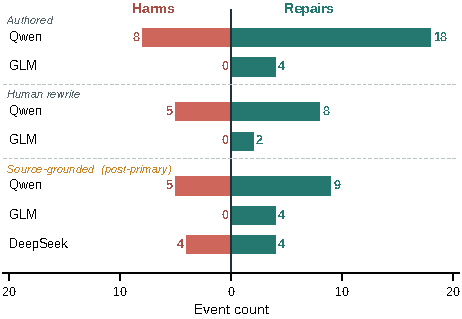
\includegraphics[width=0.82\textwidth]{Figures/fig_enforcement_repairs_harms_compact.pdf}
\caption{Row-level repairs and harms from the zero-call Decision-enforced transformation of
Decision-visible outputs. Counts are separated for the authored diagnostic, human rewrites, and
source-derived contrast. Enforcement repairs more rows than it harms for Qwen on the authored and
rewrite sets, has balanced 4/4 effects for DeepSeek source transfer, and produces no harms for GLM
in any setting.}
\label{fig:supp-enforcement-repairs-harms}
\end{figure}

\subsection{Cross-schema matched-call ablation}
This earlier post-primary ablation uses the 40 changed-winner pairs from \NewSchemaReplication{}.
Each task makes one shared compiler call and two actor calls. Both actors receive the instruction,
$S_0$, the observable initial selection, $S_1$, selector, action, and action schema; the
Decision-visible actor alone receives the parsed compiler decision. A deterministic
Decision-enforced outcome reuses the visible actor call and adds no request. The first Qwen smoke
returned empty content because provider reasoning exhausted the 500-token cap. Those four failed
rows are retained as infrastructure provenance. The corrected run explicitly disables thinking
and changes no task, prompt, outcome, metric, or denominator.

\begin{table}[H]
\centering
\small
\begin{tabular}{llccc}
\toprule
Model & Outcome & Changed PairAcc & E2E & Preserve substitution \\
\midrule
Qwen & History-only & 12/40 (30.0) & 52/80 (65.0) & 16/28 (57.1) \\
Qwen & Decision-visible & 20/40 (50.0) & 59/80 (73.8) & 4/28 (14.3) \\
Qwen & Decision-enforced & 17/40 (42.5) & 55/80 (68.8) & 0/28 (0.0) \\
GLM & History-only & 12/40 (30.0) & 52/80 (65.0) & 12/24 (50.0) \\
GLM & Decision-visible & 24/40 (60.0) & 64/80 (80.0) & 0/24 (0.0) \\
GLM & Decision-enforced & 24/40 (60.0) & 64/80 (80.0) & 0/24 (0.0) \\
\bottomrule
\end{tabular}
\caption{Completed call/information-matched ablation (post-primary). Values in parentheses are
percentages. Decision-visible minus History-only changed PairAcc is $+20.0$ points [2.5,37.5]
for Qwen and $+30.0$ [17.5,45.0] for GLM; substitution differences are $-42.9$ points
[$-61.5,-24.2$] and $-50.0$ [$-70.6,-30.0$].}
\label{tab:supp-call-matched}
\end{table}

\begin{figure}[H]
\centering
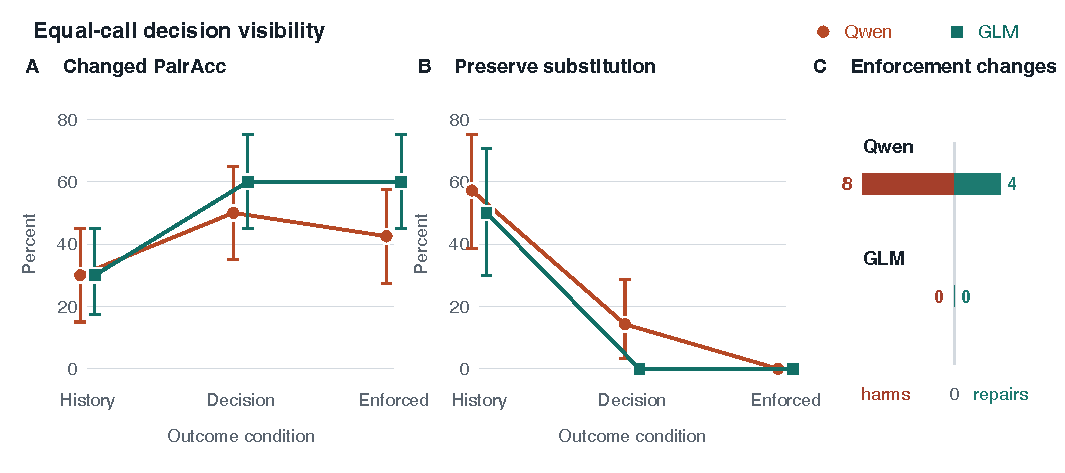
\includegraphics[width=0.96\textwidth]{Figures/tri_call_matched_ablation.pdf}
\caption{Matched-actor outcomes with state-cluster 95\% intervals. The decision block improves
joint pair accuracy and reduces Preserve substitution for both models. Enforcement introduces
Qwen harms and repairs but does not change GLM targets.}
\label{fig:supp-call-matched}
\end{figure}

The compiler predicts the correct mode on 61/80 Qwen and 64/80 GLM rows; correct Preserve binding
is 28/40 and 24/40. Qwen enforcement changes 16 outcomes, with four repairs and eight harms; its
PairAcc contrast against Decision-visible is $-7.5$ points [$-22.5,7.5$]. GLM enforcement changes
no outcome. All 480 logical calls complete without retry or parse failure. This result removes
call-count and base actor-payload asymmetry for the explicit-decision contrast, not every
difference in compiler prompting or representation.

\FloatBarrier

\subsection{Cross-Schema Replication (internal inventory: TRI-v7)}
The post-primary replication was frozen before its model calls with SHA-256 prefix
\texttt{2504f4979f1b}; the artifact manifest records the complete hash.
It contains 240 tasks over ten schemas unused in the primary diagnostic or transfer set, four independently
parameterized state instances per schema, and balanced binding, update, and explicitness factors.
All old targets remain present and action-valid. We resample the 40 state-instance clusters.

\begin{table}[h]
\centering
\small
\begin{tabular}{llrrrrr}
\toprule
Model & Controller & E2E target & Initial bind & Cond. subst. & Wrong writes & Stable err. \\
\midrule
Qwen3.5 & Generic & 47.5 & 107/120 & 43/72 & 44/240 & 4/40 \\
Qwen3.5 & Historical CTA & 70.8 & 103/120 & 0/71 & 8/240 & 6/40 \\
Qwen3.5 & Gated & 71.2 & 95/120 & 0/64 & 17/240 & 9/40 \\
GLM-5.1 & Generic & 70.0 & 120/120 & 38/80 & 38/240 & 2/40 \\
GLM-5.1 & Historical CTA & 94.2 & 104/120 & 0/70 & 14/240 & 0/40 \\
GLM-5.1 & Gated & 97.1 & 119/120 & 0/79 & 7/240 & 0/40 \\
DeepSeek-V4-Pro & Generic & 73.8 & 119/120 & 59/79 & 60/240 & 0/40 \\
DeepSeek-V4-Pro & Historical CTA & 91.2 & 107/120 & 0/70 & 17/240 & 1/40 \\
\bottomrule
\end{tabular}
\caption{Frozen new-state replication with distinct denominators. E2E target uses all 240 rows;
initial binding uses 120 anchored rows; conditional substitution requires a correct binding, a changed
winner, and a still-valid old entity; wrong writes count all non-gold mutations; stable error uses
40 anchored Stable controls.}
\end{table}

Generic conditional substitution is 59.7\% for Qwen, state-cluster 95\% CI [46.5,72.4], and
47.5\% for GLM [35.0,61.3]. CTA-minus-Generic overall differences are +23.3 points
[16.2,30.4] and +24.2 [19.6,28.7]. Fixed-executor replay instantiates all 43 and 38 Generic core
substitutions as wrong-entity writes. CTA/Gated produce zero core substitution writes after a correct binding, but
still produce 8 and 17 Qwen wrong writes, respectively, and 14 and 7 GLM wrong writes,
respectively, from opposite-mode or selector errors. Thus
the replication supports the conditional phenomenon and commitment compilation, not general
write safety. The original six Qwen/GLM 240-row runs contain zero API, parse, or internal errors.
GLM CTA records one successful transport retry; the other five runs record none.

The later DeepSeek run uses the same frozen 240 tasks and inference settings. Generic substitutes
on 59/79 opportunities, 74.7\% with state-cluster interval [62.5,86.1], while CTA substitutes on 0/70.
CTA-minus-Generic accuracy is +17.5 points [10.8,23.3]. Fixed-executor replay instantiates all 59
Generic core substitutions as wrong-entity SQLite writes. Across all errors, Generic and CTA produce 60 and 17 wrong writes;
CTA's remaining errors are outside the conditional-substitution definition. Both 240-row files have zero
API/parse errors and zero retries.

\begin{table}[h]
\centering
\scriptsize
\setlength{\tabcolsep}{2.2pt}
\begin{tabular}{lrrrr}
\toprule
Model & Shared subst. G/C & Generic PairAcc & CTA PairAcc & CTA$-$G \\
\midrule
Qwen3.5 & 41/66; 0/66 & 7/80 [2.5,16.2] & 31/80 [26.2,51.2] & +30.0 [16.2,43.8] \\
GLM-5.1 & 30/70; 0/70 & 15/80 [8.8,30.0] & 66/80 [73.8,90.0] & +63.7 [52.5,75.0] \\
DeepSeek & 50/69; 0/69 & 17/80 [11.2,32.5] & 64/80 [70.0,88.8] & +58.8 [43.8,72.5] \\
\bottomrule
\end{tabular}
\caption{Post-primary zero-API \NewSchemaReplication{} audit. Shared substitution uses only tasks where Generic and CTA
both expose the correct initial ID; G/C denotes Generic/CTA. PairAcc entries give counts and
state-cluster bootstrap 95\% intervals in percent; the final column is the paired percentage-point
difference. Zero observed CTA substitutions do not establish zero population risk.}
\label{tab:supp-shared-eligible-pairacc}
\end{table}

\subsection{Matched Full-History Baselines}
After the \NewSchemaReplication{} and DeepSeek results were known, we froze a separate strong-baseline protocol on the
unchanged 240 tasks. \texttt{interactive} is an ordinary two-call trajectory: the first response
requests refresh and the second retains the complete conversation, without TRI or reference-mode
terminology. \texttt{full\_history\_once} is a strong one-call late-authorization baseline that sees both
states and is explicitly asked whether to preserve, reevaluate, or reject. Historical CTA uses the
existing matched replication run. Temperature is zero, thinking is disabled, and the output cap is 1,200.

\begin{table}[h]
\centering
\scriptsize
\setlength{\tabcolsep}{3pt}
\begin{tabular}{lrrrrrr}
\toprule
Model & Interactive & Aware & CTA & Int. subst. & Aware subst. & CTA--Aware CI \\
\midrule
Qwen3.5 & 63.3 & 69.6 & 70.8 & 77/80 & 56/80 & +1.2 [-6.7,9.2] \\
GLM-5.1 & 67.1 & 80.8 & 94.2 & 74/80 & 38/80 & +13.3 [8.8,17.9] \\
DeepSeek & 68.8 & 75.8 & 91.2 & 68/80 & 42/80 & +15.4 [9.2,21.7] \\
\bottomrule
\end{tabular}
\caption{Matched \NewSchemaReplication{} exact-target accuracy (\%) and anchored changed-winner substitutions.
Intervals resample 40 state clusters. For Qwen, the CTA--Aware interval includes zero.}
\end{table}

All six files contain 240 rows and zero final API/parse failures. Qwen aware uses 269 request
attempts with 29 retries; the other one-call aware runs use 240 attempts and zero retries.
Interactive runs use 480 attempts. Since neither full-history condition exposes a separately
scored pre-refresh selection, its substitution rate is unconditional and is not a conditional
substitution estimate.
SQLite replay converts the interactive errors into 87/79/75 wrong writes and the aware errors
into 70/46/57 wrong writes for Qwen/GLM/DeepSeek, with four invalid attempts and one unnecessary
rejection across all six runs. Thus complete history and a late semantic reminder do not remove
wrong-entity consequences consistently across controllers; Qwen's statistically indistinguishable
comparison means the result does not
establish universal CTA superiority or pre-refresh necessity.

\section{Qualitative Trace Cases}
Table~\ref{tab:qualitative-cases} places positive, negative, and excluded cases side by side.
All rows are extracted from frozen raw outputs and executable state diffs, but were selected after
the complete runs for explanation. They demonstrate that the reported behaviors occurred in the
tested model--tool loops; they are not a random sample or evidence of natural prevalence.

\begin{table}[h]
\centering
\footnotesize
\setlength{\tabcolsep}{2.5pt}
\begin{tabular}{@{}p{0.12\textwidth}p{0.34\textwidth}p{0.25\textwidth}p{0.20\textwidth}@{}}
\toprule
Case & User instruction (abridged only for layout) & Observable model/tool trace & Classification \\
\midrule
Schema / Qwen & Choose the earliest incomplete reminder from the present view; reload; keep that chosen reminder as the action target. & bind \texttt{REM-1A} $\rightarrow$ target/write \texttt{REM-1B} & Post-binding substitution; controlled SQLite \\
TS / GLM & Before synchronizing, find the newest-created editable reminder; afterward move that reminder, without switching entries. & bind \texttt{REM-A} $\rightarrow$ \texttt{postpone(REM-B)} & Post-binding substitution; custom, post-hoc case \\
AW / GLM & Find the earliest task in the list as it is now; synchronize, then postpone the task found. & bind \texttt{6334} $\rightarrow$ \texttt{postpone(6334)} & Eligible opportunity; no violation \\
AW / Qwen & Find the alphabetically first note as the notes are now; synchronize, then append to the note found. & sync $\rightarrow$ late bind/write \texttt{3086} & Tool-order error; not TRI \\
\bottomrule
\end{tabular}
\caption{Source-validated qualitative cases. Exact instructions, raw model actions, full traces,
and source paths are in \texttt{reports/qualitative\_trace\_cases.json}. The external rows use
custom tasks on ToolSandbox-compatible (TS) or AppWorld-backed (AW) environments and are not
official benchmark results.}
\label{tab:qualitative-cases}
\end{table}

\paragraph{Frozen cross-schema write trace.}
Task \path{tri-v7-core-reminders-s1-explicit_anchor-name_collision} asks Qwen3.5 Generic
to choose the earliest incomplete reminder now, reload, and postpone that same reminder.
In $S_0$, \texttt{REM-1A} (display ``Renewal,'' due 110) wins; the compiled ledger records
\texttt{selected\_entity\_id=REM-1A}. In $S_1$, \texttt{REM-1A} remains present, incomplete,
and actionable, while \texttt{REM-1B} changes to due 103 and the same display ``Renewal.'' The
actor's final response is \texttt{"target\_id":"REM-1B"}. Replay executes
\texttt{mutate\_entity(target=REM-1B)} and records \texttt{wrong\_entity\_write}; CTA on the
same task emits and writes \texttt{REM-1A}. There are no API, parse, or protocol errors.
Sources are \path{runs/v7_qwen_generic_structured_ledger_then_act_full.jsonl},
\path{runs/v7_qwen_compile_then_act_full.jsonl}, and
\path{runs/v7_core_sqlite_replay.jsonl}.

\paragraph{ToolSandbox-compatible positive intervention.}
The post-hoc selected custom scenario ID is
\begin{center}
\path{ts2-newest-created-preserve-flip}.
\end{center}
GLM-5.1 Generic
searches \texttt{[REM-C,REM-A]}, records \texttt{selected\_entity\_id=REM-A}, synchronizes,
then searches \texttt{[REM-C,REM-A,REM-B]}. Although \texttt{REM-A} remains editable,
it calls \texttt{postpone\_reminder(REM-B)} and the database diff records a wrong write.
Matched Lifecycle writes \texttt{REM-A}. This uses ToolSandbox's reminder database and native
tools, but it is a custom benchmark-compatible intervention, not an official score. Source:
\path{runs/toolsandbox_tri_matched_glm_heldout_v1.jsonl}.

\paragraph{Opportunity without violation.}
In custom AppWorld task \texttt{appworld-todoist-p1-preserve-flip}, GLM binds task
\texttt{6334} before synchronization; new task \texttt{6336} becomes earliest afterward, but
the trace calls \texttt{postpone\_task(task\_id=6334)}. Thus a changed-winner opportunity need
not produce a violation. Source:
\path{runs/appworld_tri_Pro_zai-org_GLM-5.1_full_history_full_v1.jsonl}.

\paragraph{Excluded pre-binding write.}
Qwen task \texttt{appworld-simple-note-p1-preserve-flip} first searches, synchronizes, searches
again, and only then records refreshed note \texttt{3086} before writing it; the intended initial
target is \texttt{3084}. Because no correct pre-refresh binding exists, this is a pre-binding
tool-order error, not conditional substitution. Source:
\path{runs/appworld_tri_simple_note_Qwen_Qwen3.5-122B-A10B_full_history_full_v1.jsonl}.
The source-derived compact fields and traces for all four cases are in
\path{reports/qualitative_trace_cases.json}.

The Qwen 40-task SQLite run gives Generic Structured Ledger 27/40 final states and 13
wrong-entity writes; the GLM run gives 26/40 and 8 wrong-entity writes. A conditional audit
requires a correct initial binding, an anchored flip/name-collision update, continued presence
and action-validity of the old entity, and a final write to the refreshed winner. Under this
strict definition, core substitution writes occur in 8/8 Qwen and 6/8 GLM opportunities, versus 0/4
stable controls for each model. The remaining 5 and 2 wrong writes follow removal or invalidation
and are reported separately as reject-policy errors. On Qwen, Generic
plus a validity-only gate remains 27/40, while Lifecycle-free and Lifecycle-Gated reach 40/40.
The separately run GLM Lifecycle-Gated replay also reaches 40/40; GLM Lifecycle-free was not
run on SQLite. All reported 40/40 cells have zero wrong writes and collateral modifications. These
controlled mutation results condition on correct compilation of the lifecycle record.

\section{External Boundary Check}
\subsection{Source-derived matched-call contrast}
This post-primary protocol was frozen before its own calls. It contains 30 changed-winner pairs,
ten each grounded in STATE-Bench, AgentDojo, and ToolSandbox states and tool schemas. The refresh
and opposite-gold instructions are author-supplied controlled interventions over those source
substrates. Each model--task record uses one shared compiler call and two actors with
equal base payloads and call counts. Decision-enforced is computed offline.

\begin{table}[H]
\centering
\small
\begin{tabular}{llrrrr}
\toprule
Model & Outcome & PairAcc & E2E & Preserve subst. & Wrong writes \\
\midrule
Qwen & History-only & 12/30 & 39/60 & 7/26 & 16/60 \\
Qwen & Decision-visible & 13/30 & 39/60 & 7/26 & 17/60 \\
Qwen & Decision-enforced & 17/30 & 43/60 & 0/26 & 15/60 \\
GLM & History-only & 11/30 & 37/60 & 10/30 & 16/60 \\
GLM & Decision-visible & 20/30 & 48/60 & 1/30 & 5/60 \\
GLM & Decision-enforced & 22/30 & 52/60 & 0/30 & 4/60 \\
DeepSeek & History-only & 19/30 & 45/60 & 6/27 & 11/60 \\
DeepSeek & Decision-visible & 22/30 & 47/60 & 2/27 & 9/60 \\
DeepSeek & Decision-enforced & 20/30 & 47/60 & 0/27 & 13/60 \\
\bottomrule
\end{tabular}
\caption{Source-derived matched-call results. Preserve substitution conditions on correct
observable initial binding, a surviving actionable old target, and a distinct refreshed winner.
``Wrong writes'' counts all fixed-executor wrong-target writes, not only conditional TRI errors.}
\label{tab:supp-source-matched}
\end{table}

Decision-visible minus History-only PairAcc is +3.3 points [$-11.1$,20.0] for Qwen, +30.0
[0.0,55.6] for GLM, and +10.0 [$-10.0$,30.0] for DeepSeek. Corresponding E2E differences are
0.0 [$-6.7$,6.7], +18.3 [8.3,30.0], and +3.3 [$-5.0$,11.7]. Thus only the GLM E2E interval
excludes zero. Offline enforcement records 9/5, 4/0, and 4/4 repairs/harms for Qwen, GLM, and
DeepSeek. The complete 540 logical calls have no retry, transport failure, or parse failure.

\begin{table}[H]
\centering
\small
\begin{tabular}{lrrr}
\toprule
Source & Qwen & GLM & DeepSeek \\
\midrule
STATE-Bench & 8/10 $\rightarrow$ 8/10 & 5/10 $\rightarrow$ 10/10 & 10/10 $\rightarrow$ 9/10 \\
AgentDojo & 4/10 $\rightarrow$ 5/10 & 4/10 $\rightarrow$ 4/10 & 6/10 $\rightarrow$ 7/10 \\
ToolSandbox & 0/10 $\rightarrow$ 0/10 & 2/10 $\rightarrow$ 6/10 & 3/10 $\rightarrow$ 6/10 \\
\bottomrule
\end{tabular}
\caption{PairAcc by source, shown as History-only $\rightarrow$ Decision-visible. Null and adverse
changes are reported separately for each source.}
\label{tab:supp-source-slices}
\end{table}

\begin{figure}[H]
\centering
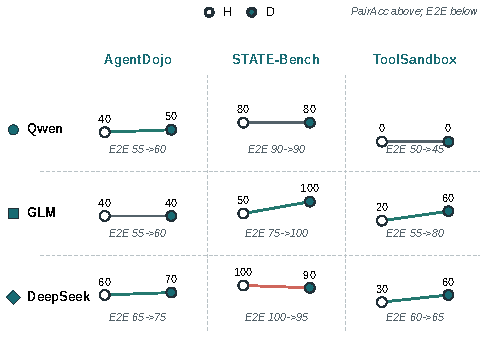
\includegraphics[width=0.68\textwidth]{Figures/fig_source_model_transfer_fingerprints_compact.pdf}
\caption{Source-derived controlled-contrast fingerprints. Open and filled points show History-only
and Decision-visible PairAcc; the text below each cell gives actionable E2E. The source--model
slices preserve the null and adverse transfers hidden by a pooled summary.}
\label{fig:supp-source-transfer-fingerprints}
\end{figure}

The event-order rule was hash-frozen before this application and reaches 15/60 exact targets and
2/30 PairAcc. The model-dependent actor results also vary across sources. Neither the fixed rule nor
timing visibility transfers uniformly across the three source-derived substrates.

\subsection{Earlier external pilots and audits}
The ToolSandbox-based 24-task pilot is exploratory and is not an official benchmark score.
For Generic, Lifecycle, Gated, and Untyped, respectively, accuracies are
79.2/87.5/91.7/91.7\% for GLM and 91.7/83.3/91.7/79.2\% for Qwen. Gated includes one GLM
and two Qwen wrong writes. It therefore demonstrates that the target-integrity diagnosis can be
instantiated in a stateful external-style tool loop, but does not establish a stable method
advantage outside the controlled TRI setting.

\paragraph{Injected checklist sensitivity.}
We tested the deterministic public-suite audit implementation using schema-shaped controls for six
suites. For each suite, five strict positives satisfy every checklist condition and five hard
negatives omit exactly one required condition. After the generator and checker were frozen, the
implementation retrieves all 30/30 positives and excludes all 30/30 hard negatives. This verifies
the code path on known labels. It does not estimate recall for naturally phrased workflows,
validate semantic candidate retrieval, or show systematic undercoverage in the public suites.

\paragraph{Model-assisted recall triage.}
A zero-API, model-assisted triage pass re-read 72 natural candidate records from ToolSandbox,
AppWorld, $\tau^3$-Bench, API-Bank, BFCL, and ToolTalk, together with 60 injected controls. It
labels 0/72 natural records as strict native opportunities while recovering all 30 strict-positive
controls and excluding all 30 hard-negative controls. We use this only as an engineering check on
candidate labeling and promptable documentation; it is not an independent recall calibration and is
not treated as additional behavioral evidence.

A post-hoc strict audit joins each trace to the frozen manifest and counts only Preserve/Flip rows
where the compiled initial ID is correct, the old entity remains present, and the refreshed winner
is a different stable ID. GLM Generic writes the refreshed winner in 3/6 opportunities, with 0/2
wrong writes on eligible Stable controls; GLM Lifecycle is 0/5. Qwen Generic is 0/6, while Qwen
Lifecycle-free is 2/6 and deterministic gate replay reduces this to 0/6. Untyped plans expose no
auditable compiled ID and are excluded from this conditional denominator. The violating GLM tasks
span newest-created, oldest-created, and alphabetically-last selectors. This is positive evidence
that TRI can occur in a benchmark-compatible database/tool substrate, but the inventory has only
six selector clusters and the strict audit was specified after the outputs existed. We therefore
report task IDs and no confirmatory interval or prevalence claim.

We then ran a separate frozen 96-task single-user-turn ToolSandbox-based extension with a
Preserve/Reevaluate $\times$ Stable/Flip design and an auditable initial-binding opportunity.
Qwen and GLM full-history agents had zero conditional substitutions in 70 and 73
opportunities; matched Qwen and GLM Generic Ledgers had zero in 64 and 87 opportunities. The
runs still produced 6, 13, 5, and 4 wrong-entity writes, respectively, but all were initial selector or tool
ordering errors and therefore excluded from the post-binding numerator. This negative external
result is retained as a boundary check rather than merged with the 24-task pilot or interpreted as
a prevalence estimate. A separate Qwen-only \texttt{generic\_state\_observed} condition is retained
in the artifact as exploratory sensitivity evidence (0/73 substitutions, six wrong writes, and
13 prohibited-schema/process errors). Its unmatched interface and protocol failures exclude it
from these four paper-facing conditions; it is not hidden or pooled with them.

\begin{figure}[H]
\centering

\includegraphics[width=0.95\textwidth]{Figures/tri_external_validity.pdf}
\caption{External validity boundary and human evidence slices.
\textbf{(A)} Public benchmark coverage audit: zero strict native opportunities under the checklist across six suites.
\textbf{(B)} Source-anchored transfer: positive evidence in one Qwen AgentDojo slice (2/7); remaining slices null.
\textbf{(C)} Human agreement by construct slice: strong support for referent core (86--98\%), weak for reject policy (55\%).
\textbf{(D)} Evidence boundary summary: the controlled diagnostic is supported; open-language generalization and natural prevalence remain unmeasured.}
\label{fig:external-validity}
\end{figure}

\subsection{Official opportunity and released-trace audit}
We audited the unmodified public inventories at the semantic-task level. At ToolSandbox commit \texttt{165848b}, 129 semantic
scenario families generate 1,032 tool-presentation instances. None contains the strict sequence
correct binding, independent external transition, and later substitutable entity mutation. One
multiple-user-turn task is TRI-like: after finding all friends and changing those stable person
IDs to enemies, ``them'' refers to the same IDs when changing them back. It has no external
refresh, competitor, or selector flip.

The downloaded AppWorld \texttt{0.1.3.post1} release contains 732 task instances from 244
generator families. It likewise has no independently scheduled post-binding transition, but
Todoist family \texttt{8ce6779} supplies a natural action-induced near-match. The Agent selects
incomplete tasks assigned to the user, reassigns them, and then must ``leave a comment there'' on
the same task IDs even though reassignment makes them fail the initial selector. We audited all
42 released trajectories for this family across 14 experiment configurations. Among 16 operations
on gold task IDs, all 16 subsequent comments preserve the same ID and none substitutes another
target. There are 152 omitted gold targets, two assignments to non-gold IDs, and three comments
on non-gold IDs; only two trajectories pass every official test. These are upstream selection and
coverage failures, not post-binding substitutions after a correct target operation.

At current $\tau^3$-Bench commit \texttt{cf71a80}, we further audit 2,449 core tasks: 50
airline, 114 retail, and 2,285 telecom. Airline and retail expose no user-side mutation during
conversation. Telecom has 2,250 tasks with user mutation actions, but none carries a customer,
line, or bill stable ID, and its single-device/app actions create no competing same-role selector
target. The strict native TRI count is therefore zero. Eight telecom tasks are natural dual-control
near-matches: the Agent binds an overdue bill, the user pays it, and the Agent resumes an
associated line. Bill and line are different referential roles, so these are not TRI. The 26
released result files contain 10,832 trajectories from GPT-4.1, GPT-4.1-mini, Claude 3.7, and
o4-mini; 936 trajectory IDs match the payment family, but none supplies a strict TRI denominator.

\begin{table}[h]
\centering
\scriptsize
\setlength{\tabcolsep}{3pt}
\begin{tabular}{lccc}
\toprule
Strict-opportunity feature & ToolSandbox & AppWorld & $\tau^3$-Bench \\
\midrule
Stable entity ID & yes & yes & no \\
Observable prior binding & yes & yes & partial \\
Independent post-binding transition & no & no & yes \\
Competing same-role entity & no & partial & no \\
Changed selector winner & no & partial & no \\
Old entity remains actionable & yes & yes & no \\
Later target mutation & yes & yes & no \\
Evaluable authorized target & yes & yes & partial \\
\bottomrule
\end{tabular}
\caption{Coverage checklist for each public benchmark's closest natural near-match, not all
tasks. ``Partial'' marks a related but non-strict structure. Every cell is justified in
\texttt{reports/benchmark\_coverage\_checklist.json}. No suite contains all required features.}
\label{tab:supp-coverage}
\end{table}

The missing conjunction can make these benchmarks unable to measure TRI; it does not show that
TRI is frequent in deployed traffic. Conversely, a near-match is evidence of task structure, not
of model violation. The source-derived funnel makes attrition explicit: ToolSandbox narrows from
129 families to 43 after entity-mutation filtering, then 26/18/1/0 after transition, prior-selection,
stable-ID, and strict-opportunity checks. AppWorld narrows from 244 families to one near-match and
zero strict exogenous opportunities; its 42 released trajectories expose 16 auditable post-binding
operations and zero substitutions. In $\tau^3$-Bench, 2,250/2,449 tasks contain a user-side mutation but
none exposes a stable ID in that mutation. These are sequential author classifications, not an
independent recall audit or a marginal feature-prevalence estimate. Full counts are generated in
\texttt{reports/public\_suite\_coverage\_funnel\_v1.json}.

A separate post-primary, zero-API structural scan parses three additional pinned test inventories:
API-Bank (528 units), BFCL multi-turn (800 variants in 200 clusters), and ToolTalk (50 dialogues).
Author-built retrieval retains 0, 57, and 23 source-anchored candidate clusters, respectively, but
finds zero strict native opportunities in each corpus. No released unit jointly exposes an observable
pre-update binding, independent refresh, surviving action-valid old target, distinct refreshed winner,
timing authorization, and target-level mutation. These are counts under the retrieval procedure,
without independent recall calibration or prevalence meaning. The 80 BFCL/ToolTalk candidates support
only further source inspection, not a native TRI positive or behavioral transfer result; the protocol,
manifest, inventory, parser, and report are included in the Code and Data Supplement.

A frozen post-primary annotation then sends each of these 80 candidates to Qwen3.5 and GLM-5.1.
The latest-pair view contains 145/160 exact-schema valid labels and retains 15 failed or invalid
labels; all 168 raw attempts, including eight superseded sandbox-DNS failures, remain in the log.
Among 65 candidates with two valid labels, 24 have a model disagreement. The strict-positive union
and intersection are both zero, while the broader source-eligible union and intersection contain
25 and one candidates. Thus no strict-positive source verification is triggered. These are fallible
model candidate labels, not independent review, recall calibration, a verified native opportunity,
a behavioral result, or a prevalence estimate.

\subsection{Frozen source-anchored external transfer}

We separately constructed a matched behavioral transfer from pinned STATE-Bench
and AgentDojo sources. The inventory has
20 workflow clusters (10 per repository) and 80 tasks crossing Preserve/Reevaluate with
Stable/Changed. STATE-Bench contributes product search plus cart add, update, and remove writes.
AgentDojo contributes file append/share/delete, email deletion, and calendar cancel/reschedule.
Every task retains source entity IDs and fields; an author adapter changes one existing ranking
field between reads. The old target remains present and action-valid. Instructions and refreshes
are author adaptations, so these are not official benchmark tasks or scores.

Two models run ordinary full history and a matched execution-record probe, yielding 320 rows.
The frozen zero-API gate passes 80/80 source-tool final-state checks. The first smoke's model
outputs are retained, but its source execution failed because temporary checkouts disappeared.
Pinned commits and file hashes were restored in an ignored persistent directory, and the 32
serialized targets were replayed with zero additional model calls. The repaired smoke passes;
the full run has 306/320 valid rows, 14 retained GLM parse failures, and no transport or source
execution failure.

% Generated by scripts/report_source_anchored_external_transfer.py.
\begin{table*}[t]
\centering
\small
\resizebox{\textwidth}{!}{%
\begin{tabular}{lllrrrrrrrr}
\toprule
Source & Model & Condition & Exact ITT & Initial & P/S & P/C & R/S & R/C & P/C$\to$new & R/C$\to$old \\
\midrule
AgentDojo & GLM & Record & 33/40 & 31/40 & 8/8 & 8/8 & 8/8 & 7/7 & 0/8 & 0/7 \\
AgentDojo & GLM & History & 33/40 & 32/40 & 8/8 & 8/8 & 8/8 & 8/8 & 0/8 & 0/8 \\
AgentDojo & Qwen & Record & 27/40 & 25/40 & 6/6 & 7/7 & 6/6 & 4/6 & 0/7 & 2/6 \\
AgentDojo & Qwen & History & 28/40 & 28/40 & 7/7 & 5/7 & 6/7 & 6/7 & 2/7 & 1/7 \\
\midrule
STATE-Bench & GLM & Record & 24/40 & 28/40 & 5/7 & 5/7 & 5/7 & 6/7 & 0/7 & 0/7 \\
STATE-Bench & GLM & History & 31/40 & 28/40 & 6/7 & 7/7 & 6/7 & 7/7 & 0/7 & 0/7 \\
STATE-Bench & Qwen & Record & 40/40 & 40/40 & 10/10 & 10/10 & 10/10 & 10/10 & 0/10 & 0/10 \\
STATE-Bench & Qwen & History & 40/40 & 40/40 & 10/10 & 10/10 & 10/10 & 10/10 & 0/10 & 0/10 \\
\bottomrule
\end{tabular}%
}
\caption{Frozen source-anchored external transfer. P/R denote Preserve/Reevaluate; S/C denote Stable/Changed. Four cell columns condition on a correct observable initial selection and a surviving action-valid old target. The final columns isolate substitution to the refreshed winner in Preserve/Changed and retention of the initial winner in Reevaluate/Changed. ITT retains parse and missing-write failures.}
\label{tab:supp-source-anchored-transfer}
\end{table*}


Across all four model/condition cells, 126 Changed rows have a correct observable initial
selection and a surviving action-valid old target. Exact-target success is 118/126. Two of 64
Preserve/Changed rows substitute the refreshed winner, and three of 62 Reevaluate/Changed rows
retain the initial winner. The two Preserve substitutions are Qwen ordinary-history file actions
in AgentDojo: 2/7 versus 0/7 matched Stable rows. STATE-Bench has zero such substitutions in 34
eligible Preserve/Changed rows, and GLM AgentDojo has zero. Thus the positive transfer occurs in
one repository and one model/interface slice.

The execution record does not provide a stable method gain. On shared correct-initial-selection
rows, ordinary history versus execution record scores 57/59 versus 52/59 for GLM and 62/65 versus
63/65 for Qwen. Cluster bootstrap estimates execution-record minus ordinary exact-target accuracy
at $-8.75$ points (95\% CI $[-16.25,-2.5]$) for GLM and $-1.25$ points
($[-6.25,3.75]$) for Qwen. This result supplies limited source-anchored bridge evidence for the
diagnostic while narrowing any claim that an explicit record is generally superior. It does not
establish native benchmark prevalence, natural traffic, independent human evidence, or an official
STATE-Bench or AgentDojo score.

\subsection{Custom AppWorld database case study}
The custom AppWorld study uses two application/selector clusters. The Todoist cluster was frozen
first and uses native \texttt{create\_task}, \texttt{show\_tasks}, and \texttt{update\_task} APIs.
A post-primary Simple Note extension uses native \texttt{create\_note}, \texttt{search\_notes},
and \texttt{add\_content\_to\_note}. Each cluster crosses Preserve/Reevaluate, Stable/Flip, and
two paraphrases. Todoist selects the earliest-due incomplete task; Stable adds a later task and
Flip an earlier one. Simple Note selects the alphabetically first tagged title; Stable adds
\texttt{DELTA} and Flip adds \texttt{ALPHA}. Old targets remain present and editable. Gold is
computed from stable IDs, and evaluators compare post-sync and final database snapshots without
an LLM judge.

\begin{table}[h]
\centering
\scriptsize
\setlength{\tabcolsep}{2pt}
\begin{tabular}{llrrrrr}
\toprule
App & Agent & Strict & Write & Bind & Subst. & Wrong \\
\midrule
Todoist & Qwen3.5 & 6/8 & 8/8 & 6/8 & 0/6 & 0 \\
Todoist & GLM-5.1 & 8/8 & 8/8 & 8/8 & 0/8 & 0 \\
Simple Note & Qwen3.5 & 6/8 & 7/8 & 6/8 & 0/6 & 1 \\
Simple Note & GLM-5.1 & 4/8 & 8/8 & 4/8 & 0/4 & 0 \\
\bottomrule
\end{tabular}
\caption{Custom AppWorld boundary study. Across 24 correct, correctly timed bindings, conditional
substitution is 0/24. The one Simple Note wrong write follows synchronization before binding and is excluded
from that denominator. Explicit sidecar omission causes the remaining strict failures. This is not
an AppWorld leaderboard result; each app contributes one selector cluster.}
\end{table}

A post-primary lower-intervention addendum removes \texttt{record\_binding} and all prompt
language about TRI, binding, or temporal authorization. Each ordinary selector API returns one
stable ID, which is logged automatically as the binding event. Across 32 Qwen/GLM trajectories,
strict success is 28/32, gold-target writes are 30/32, and conditional substitution is 0/28 (0/6 in
Preserve/Flip). Qwen's two wrong writes use the same Preserve wording in both apps: it synchronizes
before its first selector call, then writes the refreshed winner. Matched Stable rows exhibit the
same order defect but happen to write A because the winner is unchanged. This is a reproducible
pre-binding temporal-order failure and illustrates why Stable controls and a conditional-substitution
denominator are both necessary.

\section{Negative Compositional Stress Tests}
The frozen Qwen two-refresh multi-referent stress test contains 40 SQLite tasks with two refreshes, a monitoring
referent, an unrelated tool call, and a final mutation. Generic obtains 32/40 final states,
one wrong write, and four unnecessary rejections. Scalar Lifecycle obtains 28/40, six wrong
writes, six unnecessary rejections, and one parse/internal error. The difference is $-10.0$
points with a template-cluster interval of $[-35.0,12.5]$. Lifecycle mode accuracy is only
25/40: its scalar record confuses monitoring and action-target roles.

A frozen role-indexed held-out addendum then tests 40 tasks from four unseen schemas. In the
matched scalar-versus-role comparison, Qwen improves from 35/40 to 39/40 final states
(difference +10.0, cluster CI [+2.5,+20.0], McNemar $p=.21875$). GLM intention-to-treat is
40/40 scalar versus 37/40 role-indexed because three role runs fail in transport; a serial
recovery sensitivity gives 40/40 for both. Against historical CTA, Qwen obtains 38/40 versus
39/40 final states (33/40 vs. 39/40 target accuracy), and recovered GLM ties at 40/40. These results motivate role indexing but do not support
stable superiority over simpler compilation.

\section{Post-Primary Method-Upgrade Go/No-Go}
After the scalar and compositional results above were known, we froze a 20-task decision set:
16 \NewSchemaReplication{} tasks over 16 state clusters and four multi-refresh/role tasks. We reused the
matching frozen Generic, Historical CTA, Lifecycle, and role-indexed outputs and newly ran an Event
Graph compiler (M1) and Event Graph plus Executable Selector (M2) with both models. This is an
exploratory method-selection smoke, not a powered confirmatory comparison.

\begin{table}[h]
\centering
\small
\begin{tabular}{llrrrr}
\toprule
Model & Method & Correct & Schema & Mode & Selector \\
\midrule
Qwen3.5 & Event Graph & 9/20 & 14/20 & 12/20 & -- \\
Qwen3.5 & Executable Selector & 15/20 & 15/20 & 14/20 & 15/20 \\
GLM-5.1 & Event Graph & 20/20 & 20/20 & 20/20 & -- \\
GLM-5.1 & Executable Selector & 18/20 & 18/20 & 18/20 & 19/20 \\
\bottomrule
\end{tabular}
\caption{Post-primary 20-task method-upgrade smoke. Selector reports equivalence on both initial
and final states. Parse/schema failures count as incorrect under intention-to-treat.}
\end{table}

On the same combined tasks, Historical CTA obtains 13/20 for Qwen and 20/20 for GLM. M2 therefore
changes accuracy by +2 and $-2$ tasks, respectively, and fails the predeclared requirements that
both models reach at least 95\% schema/selector equivalence and show a consistent direction.
We do not promote M1 or M2 to the main method. Historical CTA remains the minimal scalar realization, while the
independently frozen role-indexing evidence above motivates role indexing as a limited compositional
extension. The zero-API oracle executor is 440/440 across the primary, cross-schema, and compositional inventories and blocks all stale/wrong writes
in 120 deterministic concurrency sequences; this establishes implementation sufficiency only,
not learned compiler performance.

\paragraph{Leave-group-out sensitivity.}
On the 240-task \NewSchemaReplication{}, we recompute the matched CTA-minus-Generic difference after
excluding one complete domain or one complete template family. The ten domain exclusions retain
ranges of 18.5--25.5, 23.1--25.9, and 15.7--22.2 points for Qwen, GLM, and DeepSeek; the sixteen
template-family exclusions retain 20.4--26.3, 20.8--26.1, and 14.2--19.6 points. Every exclusion
remains positive. This rules out dominance by one domain or template family, but does not make
templated rows independent natural-world observations.

\paragraph{Within-inventory subsampling stability audit.}
We additionally subsample complete matched clusters without replacement 10,000 times at
increasing cluster counts. This is a precision and stability diagnostic, not post-hoc power.
On \PrimaryDiagnostic{}, the audit reproduces the full Lifecycle-Gated--Generic point differences of +33.8 points
for Qwen and +28.1 for GLM; the pre-specified seed-20260717 intervals are reported in the
statistical section above. At only 10 of 20 template clusters (80 tasks), 100\% of subsamples
retain a positive difference for both models. On \NewSchemaReplication{},
the full CTA--Generic differences are +23.3 [16.2,30.4], +24.2 [19.6,28.7], and +17.5
[10.8,23.3] for Qwen, GLM, and DeepSeek. At 10 of 40 state clusters (60 tasks), positive
differences occur in 100.0\%, 100.0\%, and 99.8\% of draws; at 20 clusters all three reach
100\%. Thus the direction is stable under cluster subsampling within the observed inventory.
This does not increase the number of natural-world opportunities or justify a prevalence claim.

\paragraph{Temperature-zero repeat stability.}
Before repeat calls, we froze one balanced task from each of the 40 \NewSchemaReplication{} state clusters. The matching
subset of the original run is repeat 1; two new complete passes give three measurements for Qwen
and GLM Generic and CTA. CTA--Generic remains positive in every model-repeat cell: Qwen differences
are +25.0, +12.5, and +22.5 points, while GLM differences are +30.0, +20.0, and +25.0. Generic
conditional substitution is 5/10, 5/11, and 7/11 for Qwen and 4/12, 5/12, and 6/12 for GLM; CTA is zero
in every denominator. Exact target unanimity across all three passes is 70.0/72.5\% for Qwen
Generic/CTA and 85.0/97.5\% for GLM. Under the frozen rule this is a \textsc{Mixed} result: the
method direction and conditional mechanism are stable, but individual outputs are not fully
deterministic. The 320 new task-controller executions use 640 requests, zero retries, and 313,692
provider-reported tokens, with zero API/parse errors.

\section{Request Cost}
On the 160-task primary set, Generic uses 320 requests per model. Lifecycle-Gated uses 80
Preserve compiler calls and 160 Reevaluate compiler/actor calls, totaling 240. Mean
client-observed Qwen latency is 2.84 seconds for gated Preserve versus 3.63 for Generic
anchored tasks; corresponding GLM means are 3.47 versus 5.18 seconds. On the 40-task SQLite
set, Generic uses 80 requests and Gated uses 60. Token usage was not captured and latency is
network-dependent, so these are request-efficiency observations rather than a controlled
systems benchmark.

For the post-primary DeepSeek \NewSchemaReplication{} run, both Generic and CTA use 480 requests. Provider-reported
usage is 264,359 tokens for Generic and 216,446 for CTA; client-observed cumulative latency is
1,651.7 and 1,355.8 seconds. These matched-endpoint observations are reported for provenance,
not as a cross-provider systems claim.

\section{Blind Human Construct Validation}
One volunteer uninvolved in TRI design produced natural-language rewrites of 50 sampled scalar instructions.
The source script uses seed 20260717 and stratifies the 160-task inventory by the 20
style--update cells, selecting two or three tasks from every cell for a fixed total of 50.
Three other volunteers independently labeled 100 differently randomized original/rewrite
items. Forms used opaque IDs and concealed source task, binding mode, update, variant, and
gold. Responses were an entity ID, \textsc{Reject}, or \textsc{Clarify}; confidence was
optional. All three files contain exactly the 100 keyed IDs with no missing, duplicate,
invalid, or payload-mismatched rows.
All four participants were adults and provided informed consent. The collection instructions
described voluntary participation and discouraged names or unnecessary personal data. Two
participants received modest one-time honoraria and two were unpaid; compensation was arranged
individually and was not contingent on response content or agreement with benchmark gold.
The instructions required sufficient English to complete the English-language task, but language
background was not independently tested or retained. Recruitment channel, prior relationship to
the research team, exact honorarium amounts, and actual completion times were not recorded in the
research dataset; the administration guide estimated 45--75 minutes for rewriting and 60--90
minutes per annotator. This convenience-sample limitation precludes demographic generalization.
No formal institutional review or exemption determination was obtained. No sensitive personal
data were collected, and the anonymous Code and Data Supplement contains only de-identified
responses; private consent and study-administration records are not included.

\begin{table}[H]
\centering
\small
\begin{tabular}{lrrrrr}
\toprule
Slice & $n$ & Maj.--gold & Unanimous & $\kappa$ & $\alpha$\\
\midrule
All & 100 & 86.0 & 72.0 & .708 & .709\\
Original & 50 & 84.0 & 70.0 & .679 & .681\\
Human rewrite & 50 & 88.0 & 74.0 & .737 & .738\\
Explicit & 60 & 86.7 & 70.0 & .672 & .674\\
Implicit & 40 & 85.0 & 75.0 & .758 & .760\\
Dynamic & 50 & 98.0 & 96.0 & .924 & .925\\
Anchored actionable & 30 & 86.7 & 63.3 & .538 & .543\\
Anchored reject & 20 & 55.0 & 25.0 & .087 & .102\\
\bottomrule
\end{tabular}
\caption{Human agreement (percent except coefficients). Majority--gold uses all items, treating
six three-way ties as not matching gold. Among 94 determinate majorities, accuracy is 91.5\%.}
\end{table}

Pairwise raw agreement is 79.3\%; 4\% of items receive at least one \textsc{Clarify}. All 72
unanimous items match gold. Annotator-level gold agreement is 87\%, 80\%, and 89\%; confidence
was absent for annotator 1 and therefore is not used as an outcome. The rewrite slice does not
degrade agreement, and explicit/implicit slices are similar. The main weakness is execution
fallback: participants often preserve an invalid entity as the discourse referent while
disagreeing whether the action answer should be \textsc{Reject}. We therefore interpret the
study as support for the Preserve/Reevaluate core, not as validation of reject or conditional
policy. Complete disagreement rows and the auditable analysis script accompany the Code and Data Supplement.

\paragraph{Human-majority model sensitivity.}
Of the 50 original items, 46 have a determinate human majority, 42 majorities match benchmark
gold, and 35 are unanimously gold-aligned. Re-scoring frozen model outputs against the human
majority gives:
\begin{table}[H]
\centering
\small
\begin{tabular}{lrrr}
\toprule
Model & Generic & Lifecycle-Gated & Historical CTA\\
\midrule
Qwen3.5 & 32/46 (69.6) & 41/46 (89.1) & 42/46 (91.3)\\
GLM-5.1 & 34/46 (73.9) & 42/46 (91.3) & 41/46 (89.1)\\
\bottomrule
\end{tabular}
\caption{Accuracy against determinate human-majority targets (percent in parentheses).}
\end{table}
Gated-minus-Generic template-cluster gaps are +19.6 points with a 95\% interval of
[+5.0,+36.4] for Qwen and +17.4 [+6.8,+31.6] for GLM (18 clusters, 10,000 draws).
Secondary task-level exact McNemar tests give $p=.0117$ and $.0078$.
On the 42 majority-gold items, Gated reaches 97.6\% and 100\%; on the 35 unanimous-gold
items it reaches 97.1\% and 100\%. This sensitivity preserves the Generic-to-compiled gap but
does not show Lifecycle-Gated superiority over historical pre-refresh compilation.

\section{Independent Human-Rewrite Model Evaluation}
After the human study and before model calls, we froze 50 instructions rewritten by one
independent volunteer
and reran the unchanged four controllers. All eight files contain exactly 50 unique expected
IDs, all 400 rows have \texttt{status=ok}, and no request retry occurred.
\begin{table}[H]
\centering
\small
\begin{tabular}{lrrrr}
\toprule
Model & Generic & CTA & Lifecycle-free & Gated \\
\midrule
Qwen3.5, benchmark gold & 60.0 & 90.0 & 88.0 & 90.0 \\
GLM-5.1, benchmark gold & 74.0 & 98.0 & 92.0 & 94.0 \\
Qwen3.5, human majority & 60.4 & 89.6 & 83.3 & 85.4 \\
GLM-5.1, human majority & 68.8 & 93.8 & 83.3 & 85.4 \\
Qwen3.5, human actionable & 68.3 & 92.7 & 80.5 & 82.9 \\
GLM-5.1, human actionable & 68.3 & 92.7 & 80.5 & 82.9 \\
\bottomrule
\end{tabular}
\caption{Accuracy (\%) on all 50 rewrite golds, the 48 determinate rewrite majorities, and
the 41 majority-actionable items (excluding majority-\textsc{Reject}).}
\end{table}
On the 37 unanimous-gold rewrites, Generic/CTA/Lifecycle-free/Gated reach
75.7/97.3/86.5/89.2\% for Qwen and 81.1/100/89.2/91.9\% for GLM. On the 25 dynamic
items, CTA/Gated reach 96/80\% and 100/88\%, respectively; complete explicitness, update,
template, error-type, and majority-gold slices are in the artifact.
CTA-minus-Generic benchmark-gold differences are +30.0 points with a template-cluster
interval of [+11.3,+50.0] for Qwen and +24.0 [+8.3,+41.3] for GLM. Gated reaches the same
Qwen gold accuracy as CTA but is four points lower for GLM and lower against human majorities
for both models. Direct CTA-minus-Gated intervals are 0.0 $[-11.1,+11.1]$ for Qwen and
+4.0 $[-4.3,+14.8]$ for GLM; CTA-minus-Lifecycle-free intervals are +2.0
$[-8.5,+12.2]$ and +6.0 $[-3.6,+16.7]$, respectively. None excludes zero, so the experiment
does not establish CTA superiority over either typed variant. All five Qwen and three GLM Gated benchmark-gold errors are dynamic items
compiled as \textsc{Preserve}; one is human-contested. CTA's errors are predominantly
author-specified invalid-target outcomes. The result therefore supports pre-refresh commitment
compilation on this volunteer-authored rewrite set, not
Lifecycle-Gated superiority. The execution log discloses two pre-call empty-run failures and
the non-balanced health-smoke deviation.

\paragraph{Matched-call transfer.}
A separate post-primary run applies the full-diagnostic History-only and Decision-visible actors to
the same 50 frozen rewrites. The 50 rows form 43 clusters; only seven clusters contain both timing
modes, and only three are actionable changed-winner pairs. PairAcc is therefore a small-sample
sensitivity rather than the main endpoint.
\begin{table}[H]
\centering
\small
\begin{tabular}{llrrrr}
\toprule
Model & Outcome & Actionable E2E & Human majority & Changed PairAcc & Preserve subst. \\
\midrule
Qwen & History-only & 30/40 & 34/48 & 0/3 & 9/10 \\
Qwen & Decision-visible & 30/40 & 35/48 & 1/3 & 8/10 \\
Qwen & Decision-enforced & 33/40 & 39/48 & 2/3 & 0/10 \\
GLM & History-only & 31/40 & 33/48 & 1/3 & 9/10 \\
GLM & Decision-visible & 39/40 & 41/48 & 3/3 & 0/10 \\
GLM & Decision-enforced & 40/40 & 43/48 & 3/3 & 0/10 \\
\bottomrule
\end{tabular}
\caption{Matched-call results on one-volunteer rewrites of authored tasks. Human-majority
accuracy uses 48 determinate labels; actionable E2E excludes ten author-specified Reject rows.}
\label{tab:supp-human-rewrite-matched}
\end{table}
Decision-visible minus History-only actionable E2E is 0.0 points [$-10.0$,9.5] for Qwen and
$+20.0$ [8.6,32.5] for GLM. All 300 planned logical calls complete without transport or
parse failure. The mixed Qwen result and the three-pair changed subset are retained. This test uses
one-volunteer wording of authored semantics and is not an open-language benchmark.

\section{Model-Authored Linguistic Stress Audit}
This post-primary audit tests dependence on the authors' surface templates without treating model
output as independent human language. Before calls, we froze 24 actionable changed-winner workflow
specifications over 24 new schemas. DeepSeek-V4-Pro then wrote one Preserve and one Reevaluate
instruction per specification without seeing the original instructions, Rule* cues, controller
outputs, or entity IDs. Gold follows only from the frozen event order and states. All 48 generated
rows remain in ITT. Qwen3.5 and GLM-5.1 separately classified timing and checked selector, action,
and ambiguity; these labels are a model-assisted sensitivity, not independent annotation.

All 24 authoring calls, 96 judge calls, and 384 full controller calls completed without retry or
parse failure. Qwen accepted 25/48 instructions and GLM accepted 33/48, but their intersection
contains only 11 rows and no complete opposite-gold pair. Qwen classified 23/24 Reevaluate rows as
Preserve, while GLM classified 14/24 Preserve rows as Reevaluate. Both marked selector and action
fidelity and unambiguity true on all rows. This disagreement prevents a jointly validated PairAcc
sensitivity and is itself a construct-validity failure for model-only replacement of independent
writers and annotators.

\begin{table}[H]
\centering
\small
\begin{tabular}{llrrrr}
\toprule
Model & Controller & Row acc. & PairAcc & Preserve substitution & Failures \\
\midrule
Qwen3.5 & Generic & 24/48 & 0/24 & 24/24 & 0 \\
Qwen3.5 & CTA & 36/48 & 12/24 & 0/12 & 0 \\
GLM-5.1 & Generic & 24/48 & 0/24 & 20/24 & 0 \\
GLM-5.1 & CTA & 36/48 & 12/24 & 0/12 & 0 \\
Rule* & post-hoc & 15/48 & 5/24 & -- & 28 unresolved \\
\bottomrule
\end{tabular}
\caption{Post-primary model-authored stress audit. CTA--Generic PairAcc is +50.0 points with
state-pair bootstrap interval $[+29.2,+70.8]$ for each model. Conditional substitution requires
an exact correct initial ID. No complete pair passes both model judges, so these results do not
establish open-language transfer.}
\end{table}

The first aggregate report incorrectly scored every model row as wrong because the new
\texttt{MAS-01-A}-style IDs contain two hyphens, whereas the pre-existing normalizer retained only
\texttt{MAS-01}. The invalid all-zero report and raw rows are preserved. Before complete-set
reparsing, we froze a zero-request transport repair that accepts only a final actor
\texttt{target\_id} or compiled ID exactly equal to a serialized state ID; it uses no fuzzy,
display-name, or semantic matching. The table reports that repaired audit and is labeled
post-primary transport-repaired. The ITT direction is consistent with the controlled diagnosis,
but model-authoring and judge disagreement leave the intended open-language objection unresolved.

\section{Code and Data Supplement Map}
\enlargethispage{2\baselineskip}
The separately uploaded anonymous Code and Data Supplement contains the frozen JSONL task files, raw model outputs,
SQLite traces, report scripts, controller implementations, protocol files, SHA-256 manifests,
and tests. The directory \texttt{tri\_artifact/reports/} contains the primary
cluster reports, component audits, SQLite replay reports, ToolSandbox pilot report, and
claim-provenance records, \texttt{claims\_to\_evidence.csv}, matched-pair and qualitative-case reports, coverage checklists,
official opportunity/trace audits, and the AppWorld custom protocol.
The revision matched-call inventories, append-only execution log, raw outputs, v2 reports, and
figure generator are stored under the same \texttt{data/}, \texttt{runs/}, \texttt{reports/}, and
\texttt{scripts/} directories.
Running \texttt{PYTHONPATH=. python scripts/audit\_main\_paper\_evidence.py} rebuilds the
paper-facing evidence audit from frozen raw outputs and source reports and checks the critical
diagnostic-table rows and headline claims against the manuscript source.
Current submission runners receive credentials through environment
variables; credentials are not embedded in or stored with the artifact.

\paragraph{AI-assisted engineering disclosure.}
Generative AI systems were used for language editing, code assistance, internal review, and the
disclosed model-authored linguistic stress audit. They
were not treated as authors, citable sources, independent annotators, or independent human
evidence. The authors verified the manuscript claims, references, code, and reported results.

\paragraph{Model and environment provenance.}
The paper-facing API runs use SiliconFlow's OpenAI-compatible
\texttt{https://api.siliconflow.cn/v1/chat/completions} endpoint and the exact provider model IDs
\texttt{Qwen/Qwen3.5-122B-A10B}, \texttt{Pro/zai-org/GLM-5.1}, and
\texttt{deepseek-ai/DeepSeek-V4-Pro}. The provider did not expose immutable weight revisions or
serving hardware, which limits exact API replay. Frozen primary and cross-schema calls use temperature zero,
thinking disabled, and a 1,200-token output cap; per-row timestamps, request attempts, retries,
latency, and configuration are stored in raw JSONL. Protocol files record timeout, retry, smoke,
and stopping rules for each extension, while prompts are literal strings in the versioned
runners. Paper-facing primary and replication calls span July 17--26, 2026 (UTC). Offline reports
and tests were verified on macOS 26.5.1 arm64 with Python 3.12.13 and
pytest 9.1.1; core generation, scoring, bootstrap, and SQLite replay use the Python standard
library. These local details reproduce analysis from frozen outputs, not provider inference.

\end{document}
